\documentclass[usenatbib,useAMS,usedcolumn]{mnras}

\usepackage{newtxtext,newtxmath}

% Use vector fonts, so it zooms properly in on-screen viewing software
% Don't change these lines unless you know what you are doing
\usepackage[T1]{fontenc}

% Allow "Thomas van Noord" and "Simon de Laguarde" and alike to be sorted by "N" and "L" etc. in the bibliography.
% Write the name in the bibliography as "\VAN{Noord}{Van}{van} Noord, Thomas"
\DeclareRobustCommand{\VAN}[3]{#2}
\let\VANthebibliography\thebibliography
\def\thebibliography{\DeclareRobustCommand{\VAN}[3]{##3}\VANthebibliography}

%%%%% AUTHORS - PLACE YOUR OWN PACKAGES HERE %%%%%

% Only include extra packages if you really need them. Common packages are:
\usepackage{graphicx}	% Including figure files
\graphicspath{{fig/}}
\usepackage{amstext}
\usepackage{siunitx}
\sisetup{
separate-uncertainty,  
range-units = brackets}  
\usepackage{mathtools}
\usepackage{color}
\usepackage{twoopt}
\usepackage{hyperref} %% to avoid \citeads line fills
\usepackage{afterpage}
\usepackage{silence}
\usepackage{hyperref}

%%%%%%%%%%%%%%%%%%%%%%%%%%%%%%%%%%%%%%%%%%%%%%%%%%

%%%%% AUTHORS - PLACE YOUR OWN COMMANDS HERE %%%%%

% common astronomical symbols
\let\sun\odot
% astrophysical units
\DeclareSIUnit\lightspeed{$c$}
\DeclareSIUnit\rydberg{Ry}
\DeclareSIUnit\erg{erg}
\DeclareSIUnit\magnitude{mag}
\DeclareSIUnit\jansky{Jy}
\DeclareSIUnit\gauss{G}
\DeclareSIUnit\h{$h$}
\DeclareSIUnit\hseven{$h$_7}
\DeclareSIUnit\parsec{pc}
\DeclareSIUnit\year{yr}
\DeclareSIUnit\solarluminosity{\ensuremath{L_\sun}}
\DeclareSIUnit\solarmass{\ensuremath{M_\sun}}
\DeclareSIUnit\solarmassinenergy{\ensuremath{M_\sun|c^2}}
\DeclareSIUnit\solarradius{\ensuremath{R_\sun}}
% redeclared units
\DeclareSIUnit\arcsecond{as}
\DeclareSIUnit\astronomicalunit{au}
\DeclareSIUnit\clight{\ensuremath c}

% Please keep new commands to a minimum, and use \newcommand not \def to avoid
% overwriting existing commands. Example:
%\newcommand{\pcm}{\,cm$^{-2}$}	% per cm-squared

\bibpunct{(}{)}{;}{a}{}{,}             %% natbib format for A&A and ApJ
\makeatletter
  \newcommandtwoopt{\citeads}[3][][]{\href{http://adsabs.harvard.edu/abs/#3}%
    {\def\hyper@linkstart##1##2{}%
     \let\hyper@linkend\@empty\citealp[#1][#2]{#3}}}
  \newcommandtwoopt{\citepads}[3][][]{\href{http://adsabs.harvard.edu/abs/#3}%
    {\def\hyper@linkstart##1##2{}%
     \let\hyper@linkend\@empty\citep[#1][#2]{#3}}}
  \newcommandtwoopt{\citetads}[3][][]{\href{http://adsabs.harvard.edu/abs/#3}%
    {\def\hyper@linkstart##1##2{}%
     \let\hyper@linkend\@empty\citet[#1][#2]{#3}}}
  \newcommandtwoopt{\citeyearads}[3][][]%
    {\href{http://adsabs.harvard.edu/abs/#3}
    {\def\hyper@linkstart##1##2{}%
     \let\hyper@linkend\@empty\citeyear[#1][#2]{#3}}}
%  \renewcommand*\aa@pageof{, page \thepage{} of \pageref*{LastPage}}
\makeatother
\hypersetup{pdfpagemode = {UseNone},
            pdftitle = {The dispersal of protoplanetary discs},
            pdfcreator = {\LaTeX},
            pdfproducer = {pdfeTeX-0.\the\pdftexversion\pdftexrevision},
            pdfauthor = {Giovanni Picogna, Barbara Ercolano, Catherine Espaillat},
            pdfsubject = {},
            pdfview = {FitH},
            pdfstartview = {FitH},
            colorlinks = {true},
            linkcolor = [rgb]{0,0.35,0.7},
            citecolor = [rgb]{0,0.35,0.7},
            filecolor = [rgb]{0.61,0,0},
            urlcolor = [rgb]{0,0.35,0.7},
           }

\WarningFilter{latex}{Text page}

\newcommand{\new}[1]{{\bf \color{black} #1}}
\newcommand{\todo}[1]{{\bf \color{red} #1}}

\defcitealias{2019MNRAS.487..691P}{Paper~I}
\defcitealias{Ercolano2021}{Paper~II}

%%%%%%%%%%%%%%%%%%%%%%%%%%%%%%%%%%%%%%%%%%%%%%%%%%

%%%%%%%%%%%%%%%%%%% TITLE PAGE %%%%%%%%%%%%%%%%%%%

% Title of the paper, and the short title which is used in the headers.
% Keep the title short and informative.
\title[The dispersal of protoplanetary discs]{The dispersal of protoplanetary discs. -- III: Influence of stellar mass on disc photoevaporation}

% The list of authors, and the short list which is used in the headers.
% If you need two or more lines of authors, add an extra line using \newauthor
\author[G. Picogna et al.]{
Giovanni Picogna,$^{1}$ \href{https://orcid.org/0000-0003-3754-1639}{
\includegraphics[scale=0.04]{orcid}} \thanks{E-mail: picogna@usm.lmu.de}
Ercolano Barbara,$^{1,2}$ \href{https://orcid.org/0000-0001-7868-2740}{
\includegraphics[scale=0.04]{orcid}}
Catherine Espaillat$^{3}$ \href{https://orcid.org/0000-0001-9227-5949}{
\includegraphics[scale=0.04]{orcid}}
\\
% List of institutions
$^{1}$Universit\"{a}ts-Sternwarte, Ludwig-Maximilians-Universit\"{a}t M\"{u}nchen,
        Scheinerstr. 1, D-81679 M\"{u}nchen, Germany\\
$^{2}$Excellence Cluster Origins, Boltzmannstrasse 2, D-85748 Garching bei M\"{u}nchen, Germany\\
$^{3}$Department of Astronomy \& Institute for Astrophysical Research, Boston University, 725 Commonwealth Avenue, Boston, MA 02215, USA
}

% These dates will be filled out by the publisher
\date{Accepted XXX. Received YYY; in original form ZZZ}

% Enter the current year, for the copyright statements etc.
\pubyear{2021}

% Don't change these lines
\begin{document}
\label{firstpage}
\pagerange{\pageref{firstpage}--\pageref{lastpage}}
\maketitle

% Abstract of the paper
\begin{abstract}
The strong X-ray irradiation from young solar-type stars may play a crucial role in the thermodynamics and chemistry of circumstellar discs, driving their evolution in the last stages of disc dispersal as well as shaping the atmospheres of newborn planets.
In this paper we study the influence of stellar mass on mass-loss rates due to X-ray irradiation, extending our previous study of the mass-loss rate's dependence on the X-ray luminosity and spectrum. We focus on stars with masses between $0.1$ and \SI{1}{\solarmass}, which are the main target of current and future missions to find potentially habitable planets.
We found a linear relationship between the mass-loss rates and the stellar masses when changing the X-ray luminosity accordingly with the stellar mass.
This linear increase is observed also when the X-ray luminosity is kept fixed because of the lower disc aspect ratio which allows the X-ray irradiation to reach larger radii.
We provide new analytical relations for the mass-loss rates and profiles of photoevaporative winds as a function of the stellar mass that can be used in disc and planet population synthesis models.
Our photoevaporative models correctly predict the observed trend of disc life-time as a function of stellar mass with an increased steepness for stars smaller than \SI{0.3}{\solarmass}, indicating that X-ray photoevaporation is a good candidate to explain the observed disc lifetimes.
\end{abstract}

% Select between one and six entries from the list of approved keywords.
% Don't make up new ones.
\begin{keywords}
    accretion, accretion discs --
    protoplanetary discs --
    circumstellar matter --
    stars: pre-main-sequence --
    stars: winds, outflows --
    X-rays: stars.
\end{keywords}

%%%%%%%%%%%%%%%%%%%%%%%%%%%%%%%%%%%%%%%%%%%%%%%%%%

%%%%%%%%%%%%%%%%% BODY OF PAPER %%%%%%%%%%%%%%%%%%

%-------------------------------------------------------------------
\section{Introduction}
%-------------------------------------------------------------------

Our understanding of the physical processes driving the evolution of protoplanetary discs and ultimately the formation of planets is based on the observational evidence of disc lifetimes.

\citetads{1989AJ.....97.1451S} found that accretion discs are ubiquitous around young stellar objects (\SI{\sim 1}{Myr}). The initial disc fraction is almost independent of stellar mass (from $0.1$ up to \SI{10}{\solarmass}) and stellar environment (\citeads{2000AJ....120.3162L}, \citeads{2006A&A...451..177B}).
After \SI{10}{Myr} the picture changes completely since more than \SI{90}{\percent} of stars show no emission within \SI{1}{\astronomicalunit} \citepads{2004ApJ...612..496M}, and emission from small grains is found only in a few per cent of discs (\citeads{2004ApJ...608..526L}, \citeads{2005AJ....129.1049C}, \citeads{2006ApJ...639.1138S}).
This sets an upper limit to the disc dispersal process within $10$ to \SI{20}{Myr} (\citeads{2007ApJ...671.1784H}, \citeads{2010A&A...510A..72F}, \citeads{2014A&A...561A..54R}). Moreover, fitting the fraction of discs with dust emission at different wavelengths, \citetads{2014A&A...561A..54R} found an e-folding time of \SIrange{2}{3}{Myr} at \SIrange[]{3}{12}{\micro\meter} and \SIrange[]{4}{6}{\mega\year} at \SIrange[]{22}{24}{\micro\meter}, hinting at an inside-out dispersal of proto-planetary discs or to a second generation dust production \citepads[see also][]{2013MNRAS.428.3327K}.
The dust disc lifetime as a function of the stellar mass is less well characterised but the dispersal timescale appears to be up to two times faster for high mass stars ($\geq$ \SI{2}{\solarmass}, \citeads{2015A&A...576A..52R}).
The mass accretion onto the central star has also been studied extensively, though its evolution is less well constrained. Nevertheless, it has been shown that the characteristic timescale of disc accretion is shorter than that of dust disc dispersal (\citeads{2006ApJ...648.1206J}, \citeads{2010A&A...510A..72F}), and the accretion rate falls off as a function of time with a power law (e.g., \citeads{2012ApJ...755..154M}, \citeads{2014A&A...572A..62A}, \citeads{2016ARA&A..54..135H}).

The main physical process driving disc dispersal is still largely unconstrained, and it might change during the disc evolution and at different locations in the disc. A large body of evidence is pointing at magnetic disc winds as the main mechanism responsible for angular momentum transfer and mass-loss \citepads{2016ApJ...821...80B}, particularly at early times. Photoevaporative disc winds may also co-exist at early times and perhaps dominate at later stages (\citeads{2017RSOS....470114E}; \citeads{2020MNRAS.496..223W}). From a theoretical standpoint, there is a push to obtain better models that can be linked to observables to test their validity.

In the first paper of this series (\citeads{2019MNRAS.487..691P}, hereafter \citetalias{2019MNRAS.487..691P}) we showed the dependence between the stellar X-ray luminosity and the mass-loss rate due to thermal winds generated by the XEUV heating from the central star. Then we studied the influence of Carbon depletion \citepads{2019MNRAS.490.5596W} and stellar spectra hardness on the mass-loss rates (\citeads{Ercolano2021}, hereafter \citetalias{Ercolano2021}). In this following work, we focus on stellar mass dependence and how it might influence disc evolution.

In Section~\ref{sec:methods} we briefly discuss the numerical set-up adopted, following our previous work. We then describe the main results in Section~\ref{sec:results} and discuss the theoretical and observational implications of them in Section~\ref{sec:discussion}. The main conclusions are then drawn in Section~\ref{sec:conclusions}.

%-------------------------------------------------------------------
\section{Methods}\label{sec:methods}
%-------------------------------------------------------------------
We run a series of hydrodynamical simulations following the approach outlined in \citetalias{2019MNRAS.487..691P} that we briefly describe here for completeness.

The initial set-up is based on the gas densities and dust temperatures from the hydrostatic disc models from the D’Alessio Irradiated Accretion Disk (\textsc{diad}) radiative transfer models \citepads{1998ApJ...500..411D,1999ApJ...527..893D,2001ApJ...553..321D,2005ApJ...621..461D,2006ApJ...638..314D}, that best fit the median spectral energy distribution (SED) in Taurus. 
For this particular study a different set-up is adopted for each individual stellar mass, based on its mass and bolometric luminosity (see Fig.~\ref{fig:initdiscs}).
\begin{figure*}
    \centering
    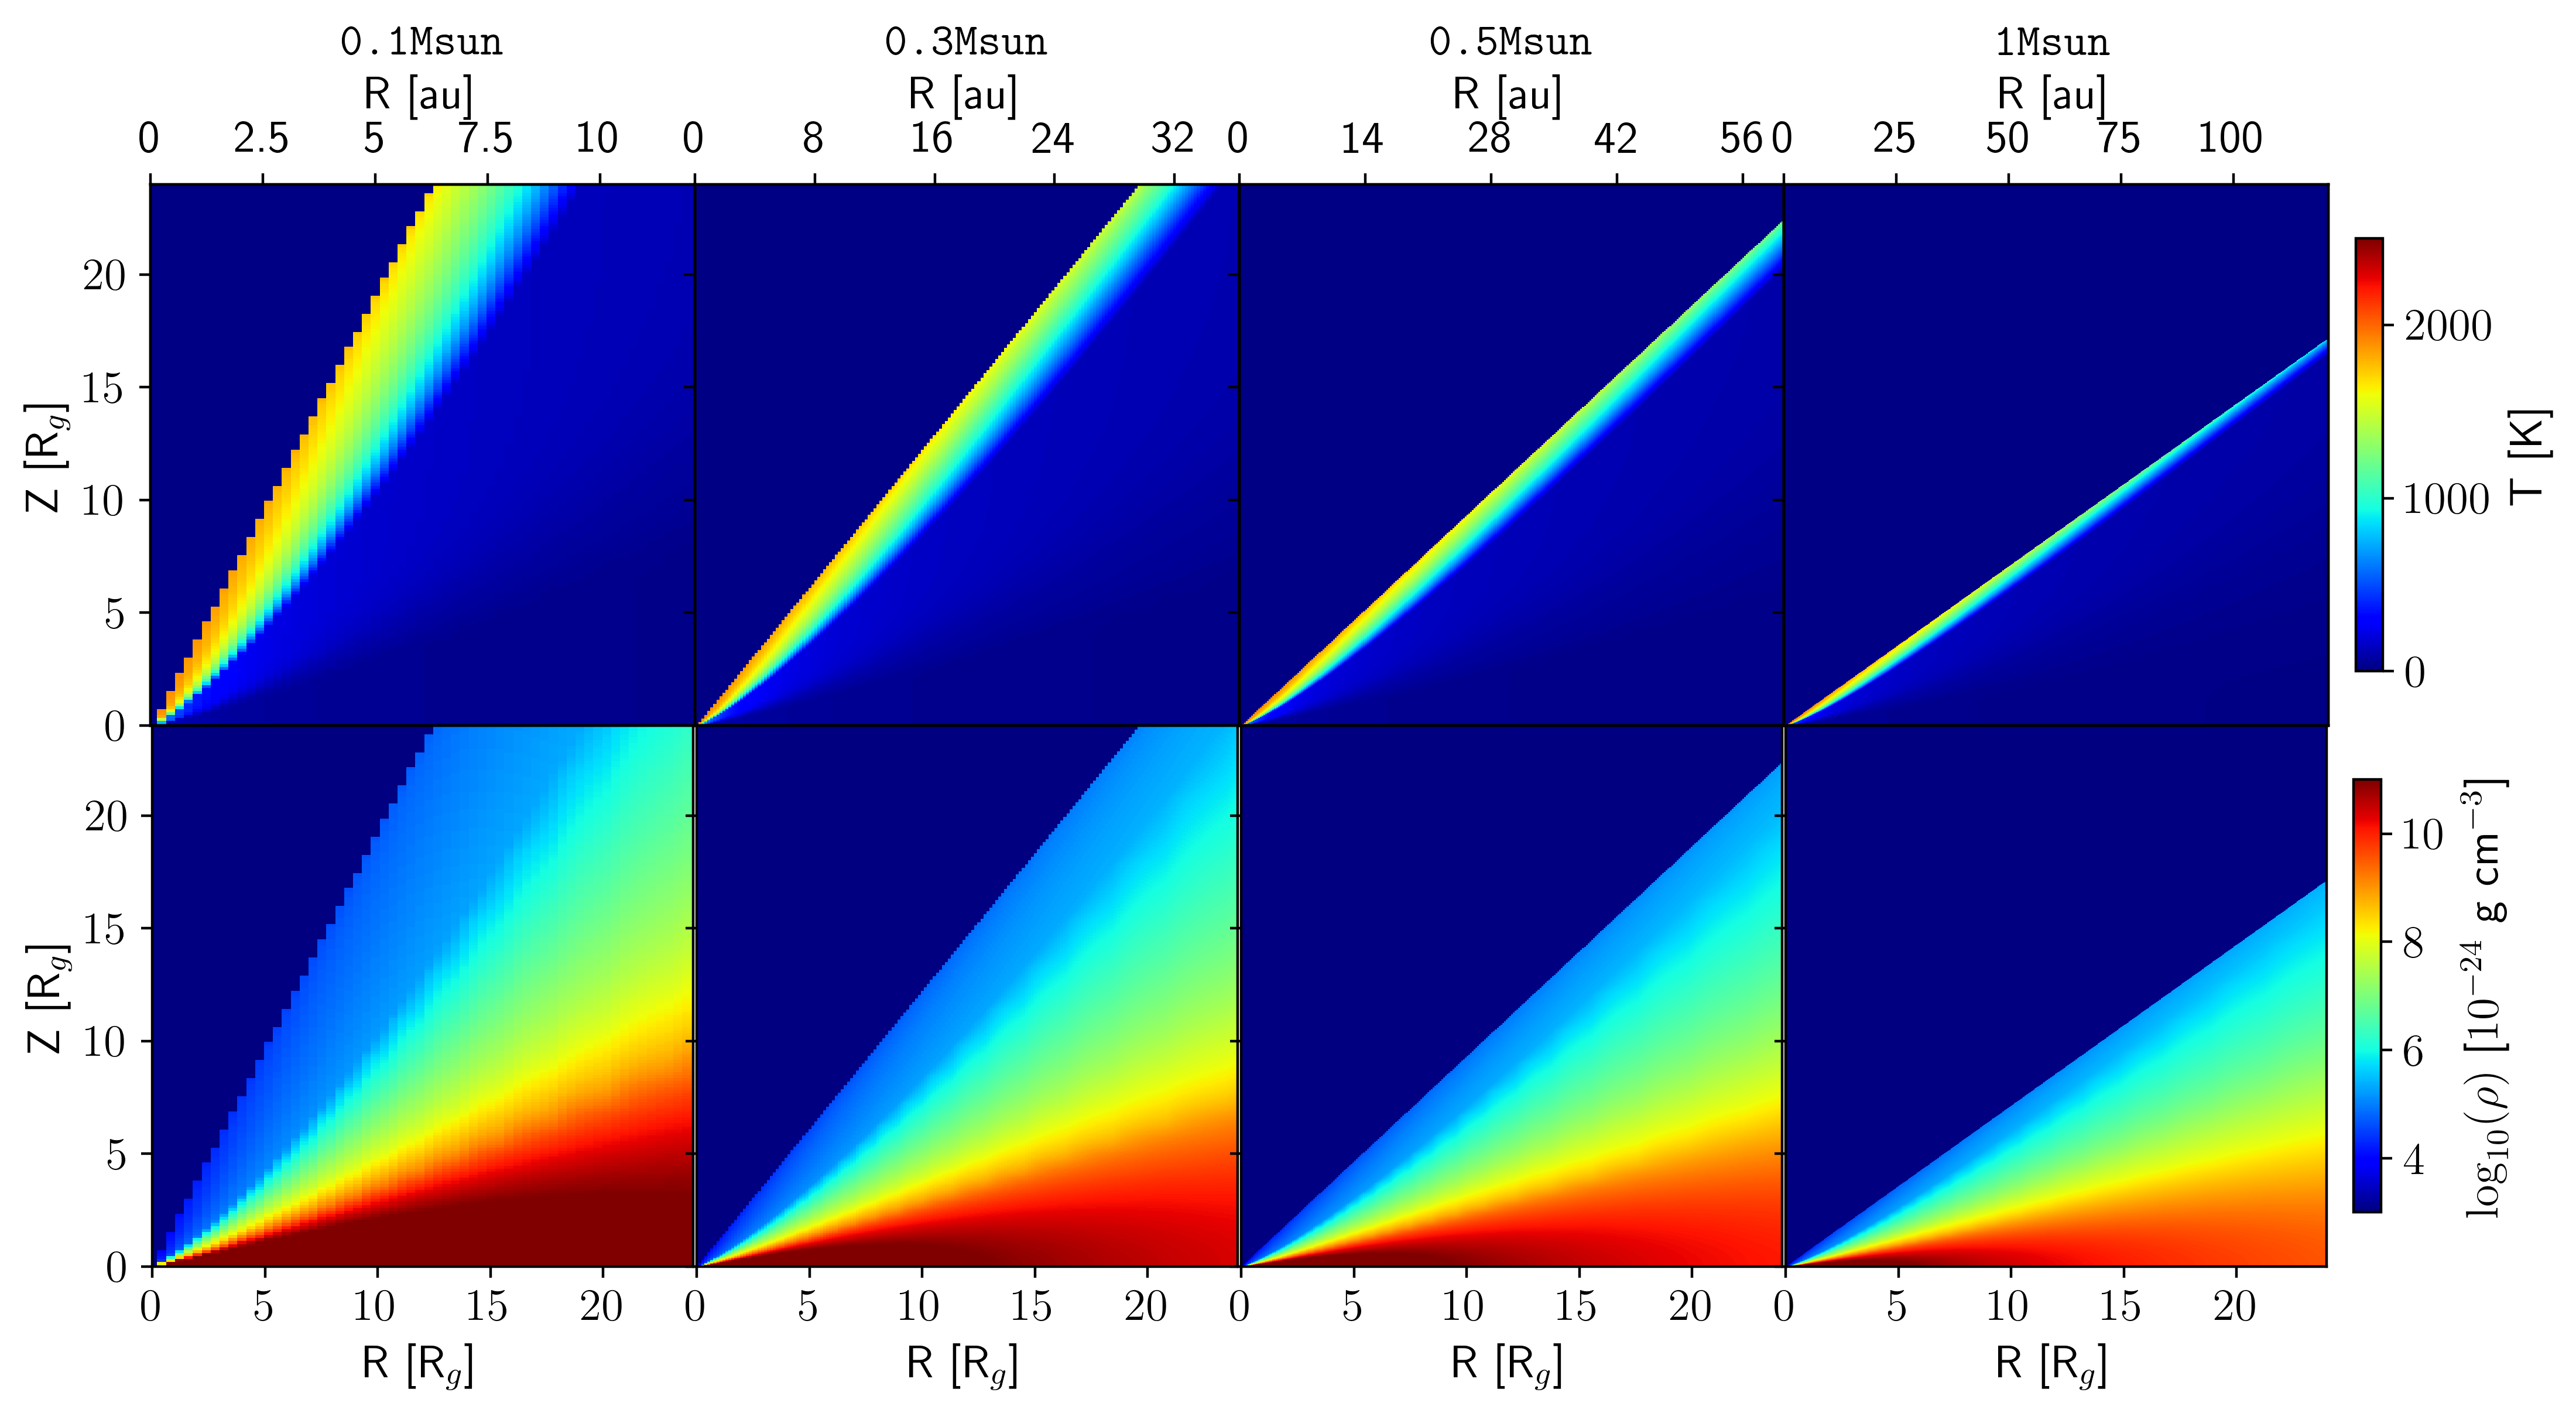
\includegraphics[width=\textwidth]{Figure1}
    \caption{Initial dust temperature (upper panel) and density (lower panel) distribution in the inner 20 gravitational radii for the the different runs from the \textsc{diad} models. \label{fig:initdiscs}}
\end{figure*}
The stellar parameters were obtained from \citetads{2000A&A...358..593S} for an age of \SI{1}{Myr}, and a metallicity $Z=0.02$ without overshooting.

We then ran the gas photoionization and dust radiative transfer code \textsc{mocassin} \citepads{2003MNRAS.340.1136E,2005MNRAS.362.1038E,2008ApJS..175..534E}, that solves the heating and cooling terms for various physical and irradiation properties at the thermal equilibrium, to obtain a temperature prescription in the upper layers of the discs when irradiated by an X(EUV) stellar spectra.
We adopted X-ray luminosities based on the stellar mass following \citetads{2007A&A...468..353G}
\begin{equation}\label{eq:Lx}
	\log_{10}{(\mathrm{L}_X)} = (1.54 \pm 0.12) \log_{10}{(\mathrm{M}_\star)} + (30.31 \pm 0.06)\,,
\end{equation}
although a recent analysis by \citetads{2021A&A...648A.121F} found a steeper dependence.

The temperature prescription is shown Figure~\ref{fig:tempxi} for the different spectral hardness (from \texttt{Spec29} corresponding to \SI{e29}{erg.s^{-1}} to \texttt{Spec31} equal to \SI{e31}{erg.s^{-1}}) following \citetalias{Ercolano2021}.
It relates the local gas temperature to the column density to the central star (from \SI{5e20}{pp.cm^{-2}} to \SI{2e22}{pp.cm^{-2}}), and the local ionization parameter \citepads{1969ApJ...156..943T}
\begin{equation}
    \xi = \frac{L_X}{n r^2}\,,
\end{equation}
where $L_X$ is the X-ray luminosity, $n$ the number density, and $r$ the spherical radius from the central star. We compared it for completeness with the previously derived temperature prescription (used in \citetalias{2019MNRAS.487..691P}) obtained for a star with $L_X=\SI{2e30}{erg.s^{-1}}$ in \citetads{2008ApJS..175..534E}.

Finally we ran a set of hydrodynamical simulations with a version of the \textsc{pluto} code \citepads{2007ApJS..170..228M} modified in \citetalias{2019MNRAS.487..691P}, in order to use the temperature prescription from \textsc{mocassin} for column densities lower than the maximum penetration depth of X-rays (\SI{\sim 2e22}{pp.cm^{-2}}), and a perfect coupling between gas and dust temperatures using the \textsc{diad} models for larger column densities.
We evolve the models until a steady state is reached for the disc structure and the gas streamlines in the wind.

We modelled $4$ different stellar masses, ranging from \SI{0.1}{\solarmass} to \SI{1}{\solarmass} which, together with the \SI{0.7}{\solarmass} studied in \citetalias{2019MNRAS.487..691P}, allow us to study in detail the stellar mass dependence on the mass-loss rates due to photoevaporative winds in T Tauri stars. The initial parameters adopted in the different runs are summarised in Table~\ref{tab:stars}.

%\subsection{Thermal calculations}\label{sec:thermal-calc}
%The gas temperatures are calculated using the gas photoionization and dust radiative transfer code \textsc{MOCASSIN} \citepads{2003MNRAS.340.1136E,2005MNRAS.362.1038E,2008ApJS..175..534E}, that solves the heating and cooling terms for various physical and irradiation properties at the thermal equilibrium.
%We irradiate a slab of gas with solar abundances \citepads{2005ASPC..336...25A} depleted by the amount locked in dust grains \citep{1996ApJ...470..893S}, using a X-ray+EUV (XEUV) spectrum (see \citetads{2008ApJ...688..398E,2009ApJ...699.1639E,Ercolano2021} for details).
%The spectrum was generated by the plasma code PINTofALE \citepads{2000BASI...28..475K}, assuming an emission distribution derived for CVn binaries \citepads{2002ASPC..277..585S} which fits Chandra spectra of T Tauri stars \citepads{2007ApJ...660.1462M}.
%We model different prescriptions for the gas temperatures based on the X-ray luminosity of the central star, following the approach of \citetalias[see][]{Ercolano2021}.
%A depletion in Carbon with respect to solar abundance can, on the other hand, have a considerable effect increasing the cumulative mass-loss rates of the photoevaporative wind \citepads{2019MNRAS.490.5596W}.

%Based on the results of \citetads{2010MNRAS.401.1415O} and \citetalias{2019MNRAS.487..691P} we parameterise the gas temperature based on gas local properties (number density, $n$) via the ionization parameter
%\begin{equation}
%    \xi = \frac{L_X}{n R^2},
%\end{equation}
%where $L_X$ is the X-ray luminosity of the central star in erg/s, and $R$ is the cylindrical radius; and column density ($N$), $T(\xi,N)$.
%We then utilise them to calculate the gas temperature up to the maximum penetration depth of the X-ray irradiation, $N = N_X = 2\cdot 10^{22}$ pp/cm$^2$, during the hydrodynamical simulations.
%We divide the parameterisation in $40$ slabs equally spaced between $N=5\cdot 10^{20}$ pp cm$^{-2}$ and $N_X$. In Figure~\ref{fig:tempxi}, taken from \citetalias{Ercolano2021}, we illustrate the behaviour of the temperature dependence on the ionization parameter for the different spectra, compared with the previous model by \citetads{2010MNRAS.401.1415O}

\begin{figure}
    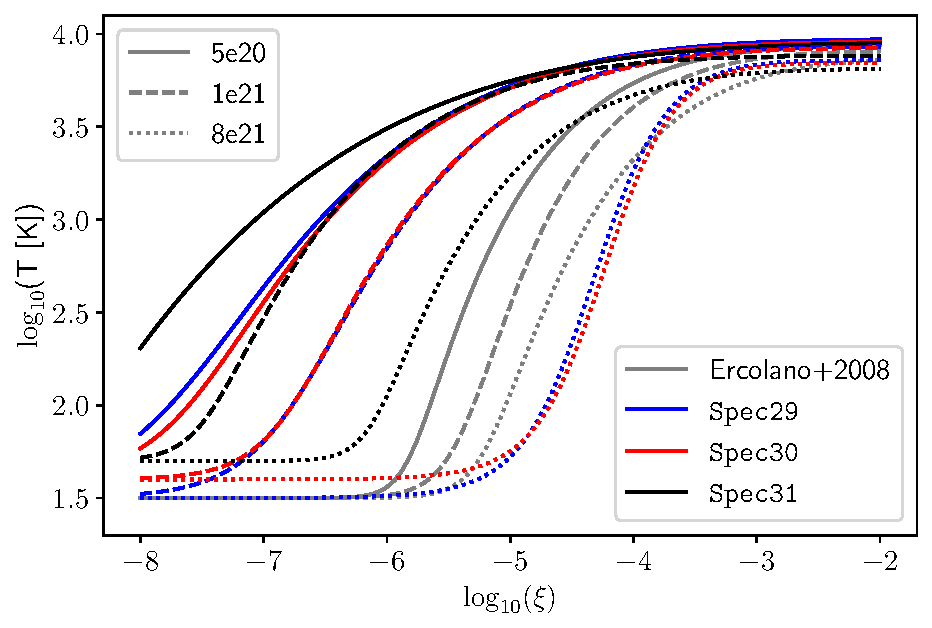
\includegraphics[width=\columnwidth]{Figure2}
    \caption{Temperature as a function of the ionization parameter, where $3$ selected column densities are highlighted \citetalias{Ercolano2021}. Three different spectral hardness are shown based on the stellar X-ray luminosity, from \texttt{Spec29} corresponding to \SI{e29}{erg.s^{-1}} to \texttt{Spec31} equal to \SI{e31}{erg.s^{-1}}.} \label{fig:tempxi}
\end{figure}

%The dust temperatures and initial density structure are calculated using the D’Alessio
%Irradiated Accretion Disk (\textsc{DIAD}) radiative transfer models \citepads{1998ApJ...500..411D,1999ApJ...527..893D,2001ApJ...553..321D,2005ApJ...621..461D,2006ApJ...638..314D}, that best fit the median spectral energy distribution (SED) in Taurus.
%The gas temperatures are assumed to be completely coupled to the dust temperature for $N>N_X$.

\begin{table*}
\caption{Star and disc properties}
\label{tab:stars}
\centering
\begin{tabular}{c c c c c c c c c c}
\hline
Name & $\mathrm{M}_\star$ [\si{\solarmass}] & $\mathrm{R}_\star$ [\si{\solarradius}] & ST & $\mathrm{L}_\star$ [\si{\solarluminosity}] & $\mathrm{L}_X$ [\SI{e29}{erg.s^{-1}}] & $\mathrm{T}_\star$ [\si{\kelvin}] & M$_\mathrm{d}$ [\si{\solarmass}] & R$_\mathrm{in}$ [\si{\astronomicalunit}] & Spectra\\
\hline
\hline
   \texttt{1Msun} & $1.0$ & $2.615$ & K6 & $2.335$ & $20.4$ & $4278$ & $0.0444$ & $0.445$ & $\mathrm{Spec30}$\\
   \texttt{0.5Msun} & $0.5$ & $2.125$ & M1 & $0.9288$ & $7.02$ & $3771$ & $0.0363$ & $0.2225$ & $\texttt{Spec30}$\\
   \texttt{0.3Msun} & $0.3$ & $2.310$ & M5 & $0.6887$ & $3.20$ & $3360$ & $0.0292$ & $0.1335$ & $\texttt{Spec29}$\\
   \texttt{0.1Msun} & $0.1$ & $1.055$ & M6 & $0.0856$ & $0.59$ & $2928$ & $0.0264$ & $0.0445$ & $\texttt{Spec29}$\\
\hline
\end{tabular}
\end{table*}

\subsection{Hydrodynamical model}\label{sec:hydro-model}

We adopted a spherical coordinate system centred on the star.
The grid is logarithmically spaced in the radial direction with \SI{500}{cells}, in order to have better resolution in the inner region of the disc (R$_\mathrm{in}=$ \SI{0.5}{R_g}), where photo-evaporation is mostly effective.
At the same time, it allows us to model the disc out to large radii (R$_\mathrm{out}$ = \SI{600}{\astronomicalunit}) without increasing strongly our computational costs and preventing boundary effects that can affect the stability of the wind flow.
For a detailed discussion of the numerical artefacts induced by the grid outer boundary, the reader is referred to \citetalias{2019MNRAS.487..691P}.
The grid is spaced linearly in the polar direction, with a refinement at the wind launching region (\SI{100}{cells} from $0.01$ to \SI{0.5}{rad}, \SI{200}{cells} from $0.5$ to \SI{1}{rad}, and $50$ cells from $1$ to $\pi / 2$ rad).
%\begin{table}
%\caption{Grid properties}
%\label{tab:hydro}
%\centering
%\begin{tabular}{c c c}
%\hline
%parameter & value & unit\\
%\hline
%\hline
%   radial range & \SI{0.05}{r_g} - $600$ & \si{\astronomicalunit} \\
%   radial resolution & $500$ & grid cells \\
%   meridional range & $0.01 - 0.5$, $0.5 - 1$, $1 - \pi/2$ & rad \\
%   meridional resolution & $100$, $200$, $50$ & grid cells\\
%\hline
%\end{tabular}
%\end{table}
We initially evolve the system for few orbits at \SI{10}{au} without stellar irradiation in order for it to readjust to the hydrostatic equilibrium. Then, we switch on the stellar heating (applied through a parameterisation as explained above and in \citetalias{2019MNRAS.487..691P}) and continue to evolve the system for a few hundred orbits until the cumulative mass-loss rate and gas streamline in the wind have reached a steady-state after few hundred orbital periods (at \SI{10}{au}), as shown in Figure~\ref{fig:mdotevol}.
\begin{figure}
    \centering
    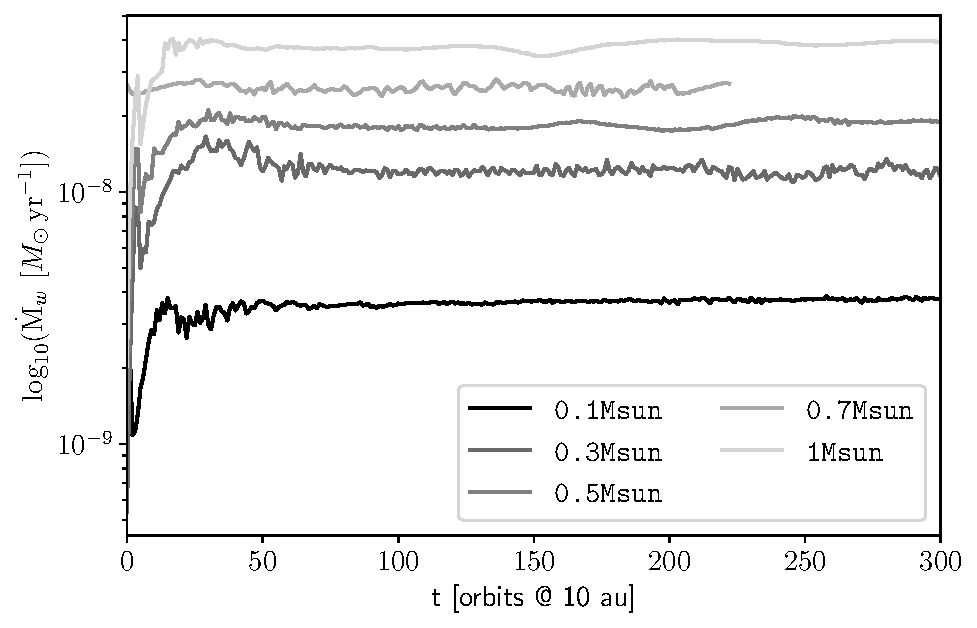
\includegraphics[width=\columnwidth]{Figure3}
    \caption{Cumulative mass-loss rate evolution as a function of time for the different stellar mass models. \label{fig:mdotevol}}
\end{figure}

%-------------------------------------------------------------------
\section{Results}\label{sec:results}
%-------------------------------------------------------------------

There are two main locations that are central in the study of photoevaporative winds.

(i) The gravitational radius $\mathrm{R}_g$, which defines the location where a gas parcel becomes unbound from the central star, equating the sound speed to the Keplerian speed (\citeads{1994ApJ...428..654H}, \citeads{2003PASA...20..337L}).
\begin{eqnarray}\label{eq:rg}
  \mathrm{R}_g &=& \frac{G \mathrm{M}_\star}{c_s^2} = \frac{\gamma-1}{2\gamma} \frac{G \mathrm{M}_\star \mu m_H}{k_B T_0} \nonumber \\ 
  &\simeq& 5.05 \left(\frac{T_0}{\SI{e4}{\kelvin}}\right)^{-1} \left(\frac{\mathrm{M}_\star}{\SI{1}{\solarmass}}\right) \ [\si{\astronomicalunit}] \,,
\end{eqnarray}
where $\gamma=5/3$ is the adiabatic index, $G$ the gravitational constant, $\mathrm{M}_\star$ the stellar mass, $\mu = 2.35$ the mean molecular weight, $m_H$ the proton mass, $k_B$ the Boltzmann constant, and $T_0$ is the temperature at the base of the flow, which is equal to \SI{e4}{\kelvin} for a pure EUV wind. Theoretically, when rescaled by the gravitational radius, stars with different stellar masses show similar wind properties. Thus we will scale in our analysis always (when not differently stated) the winds by this value, in order to study differences in the expected behaviour. We have to keep in mind that, since we are not treating an isothermal wind, the gravitational radius will not be a fixed cylindrical radius but an area where the temperature will increase due to X-ray irradiation winning over the gravitational pull from the central star. Nevertheless for simplicity in the rest of the paper we will refer to $\mathrm{R}_g$ assuming a fixed temperature of \SI{e4}{K}, typical of a isothermal EUV wind.

(ii) The critical radius $\mathrm{R}_c$, which defines the location where the gas becomes supersonic, and for a Parker wind is 
\begin{equation}\label{eq:rcrit}
    \mathrm{R}_c = \frac{G M_\star}{2 c_s^2}\,,
\end{equation}
where $c_s$ is the gas sound speed. The main assumptions of a Parker wind are that the outflow is steady, spherically symmetric and isothermal. Each streamline of the thermal wind will pass through its critical radius, forming a sonic surface which is fundamental in order to understand the properties of the photoevaporative wind. When we have the density and sound speed at the sonic surface we can determine the mass-flux in the entire flow as mass-flux is conserved (\citeads{1983ApJ...271...70B}, \citeads{2012MNRAS.422.1880O}).

In this section we discuss in the first part the effects of the irradiation from different stellar masses (and relative X-ray luminosities) on the global mass loss rates and the radial mass loss profiles obtained at steady state from our 2D hydrodynamic calculations. In the second part we isolate the effect of changing only the stellar mass (keeping fixed all the other stellar properties) and compare it with previous studies.

\subsection{Disc profiles}
We show in Fig.~\ref{fig:discs} the gas temperature (top panel) and density (bottom panel) distribution for the different stellar masses at the equilibrium.
\begin{figure*}
    \centering
    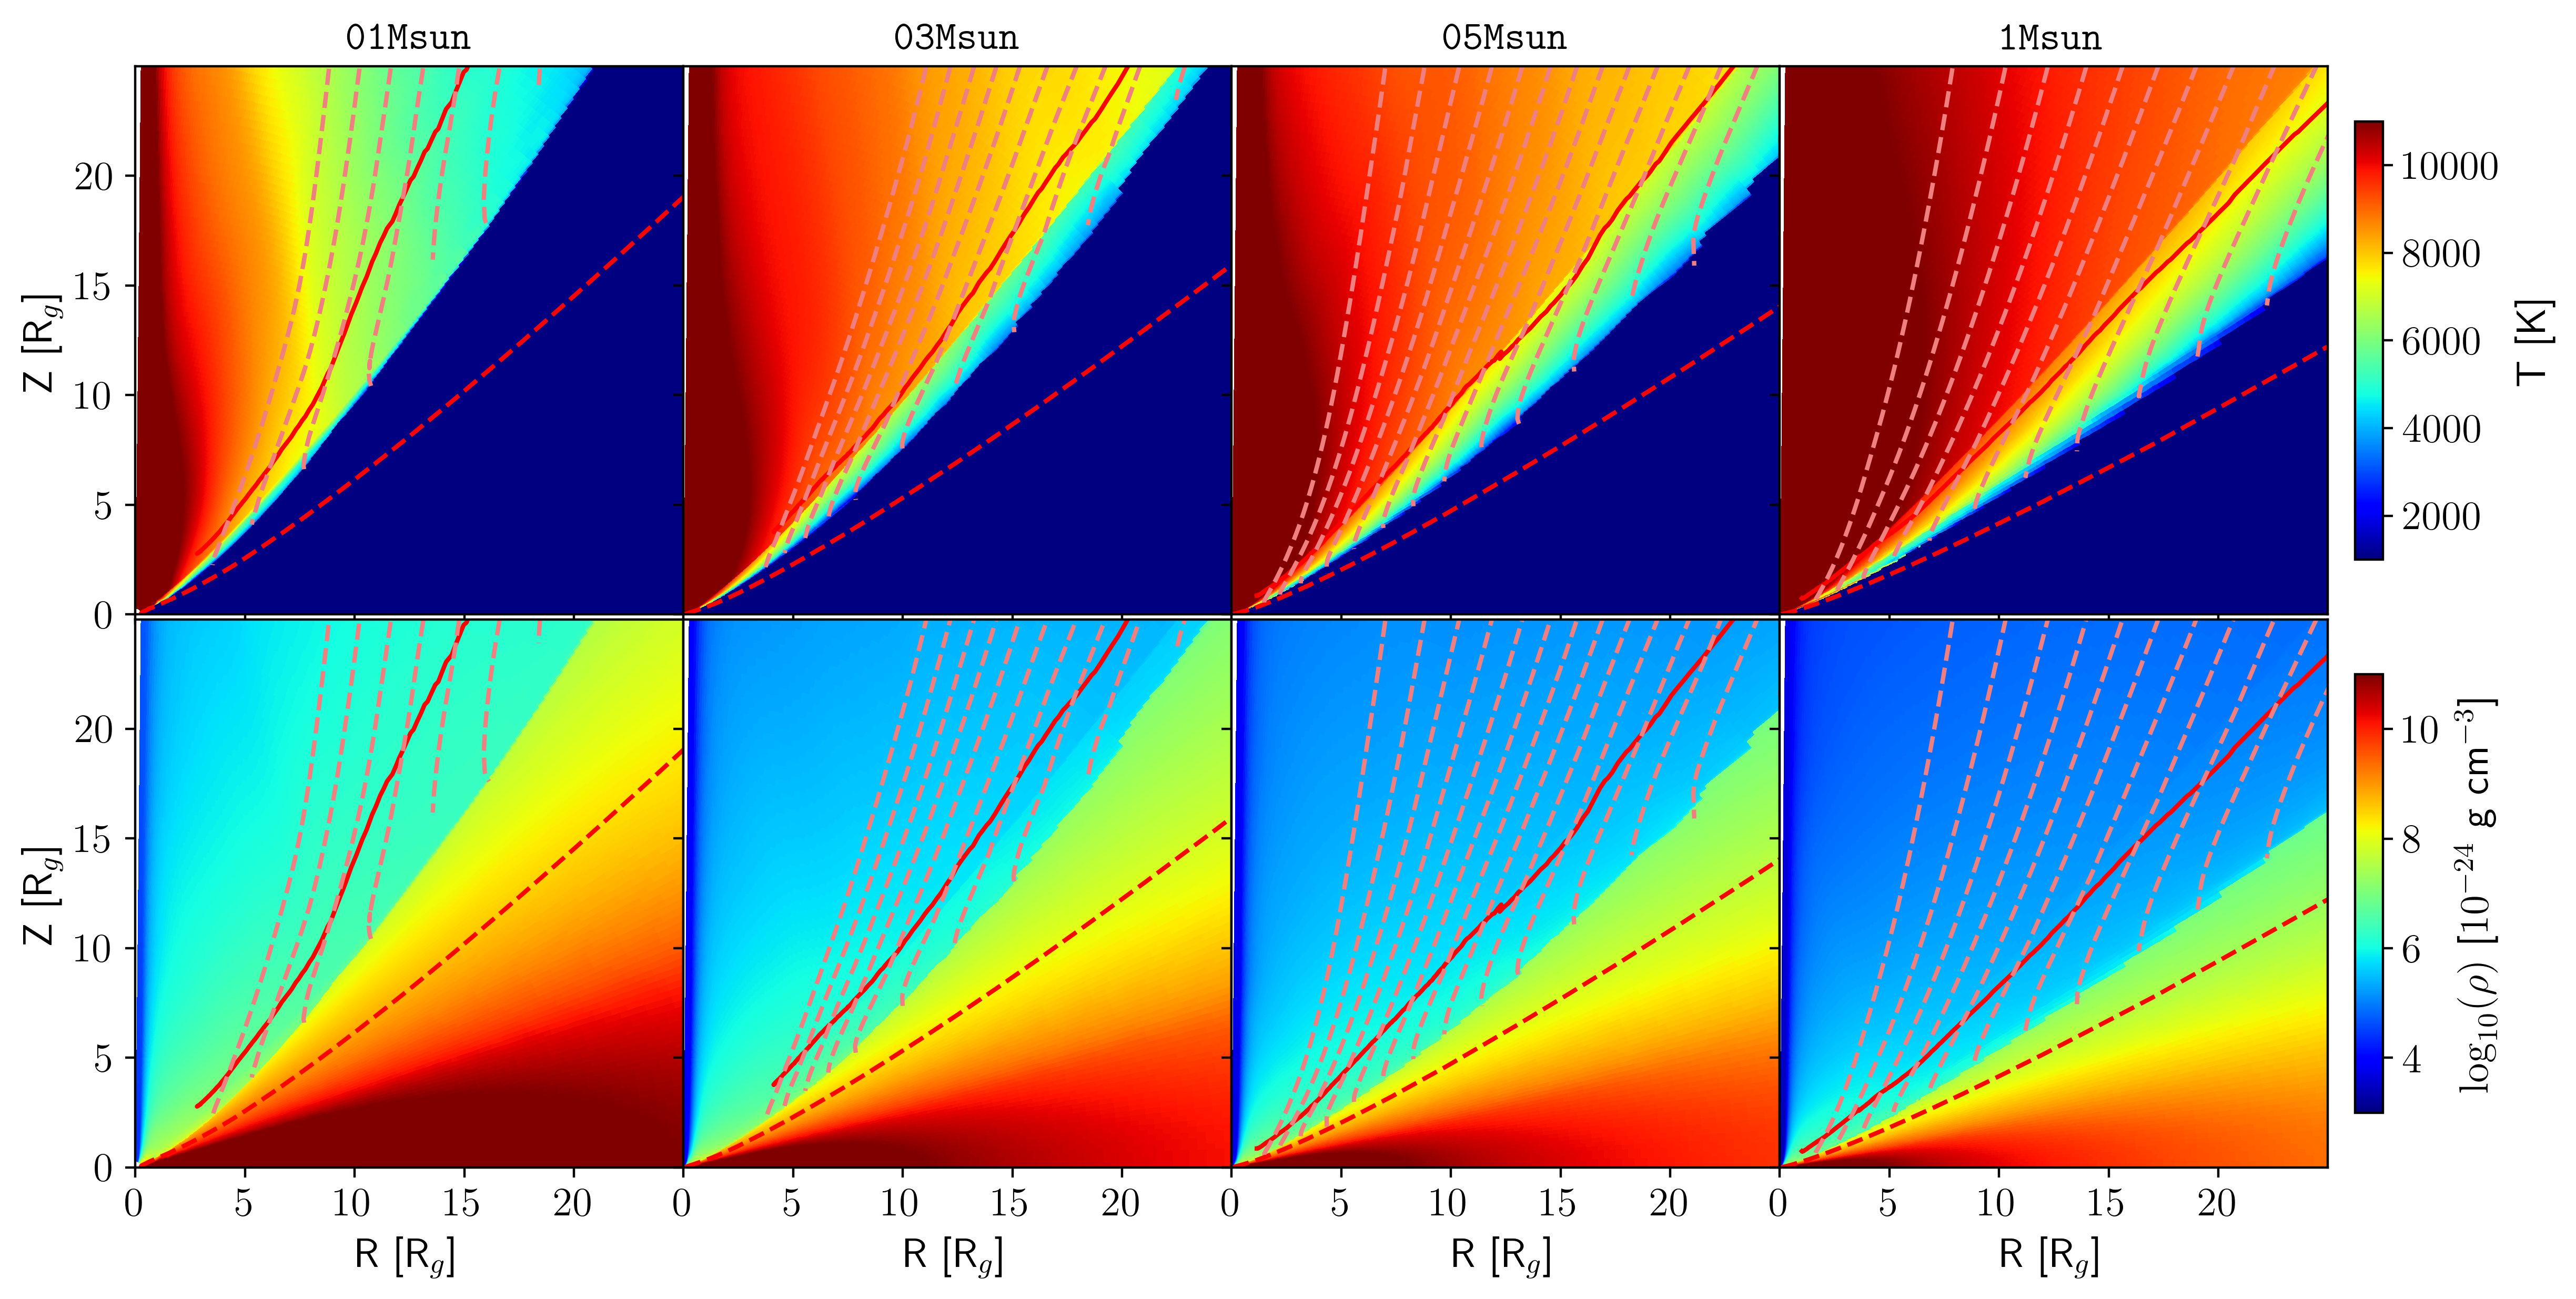
\includegraphics[width=\textwidth]{Figure4}
    \caption{Temperature (upper panel) and density (lower panel) distribution in the inner $25$ gravitational radii for the the different runs. The sonic surface is overlayed with a solid red line and the gas streamlines every $5\%$ of the cumulative mass-loss rate with orange dashed lines. The maximum penetration depth of the X-rays is shown as well with a dashed red line. \label{fig:discs}}
\end{figure*}
\begin{figure}
    \centering
    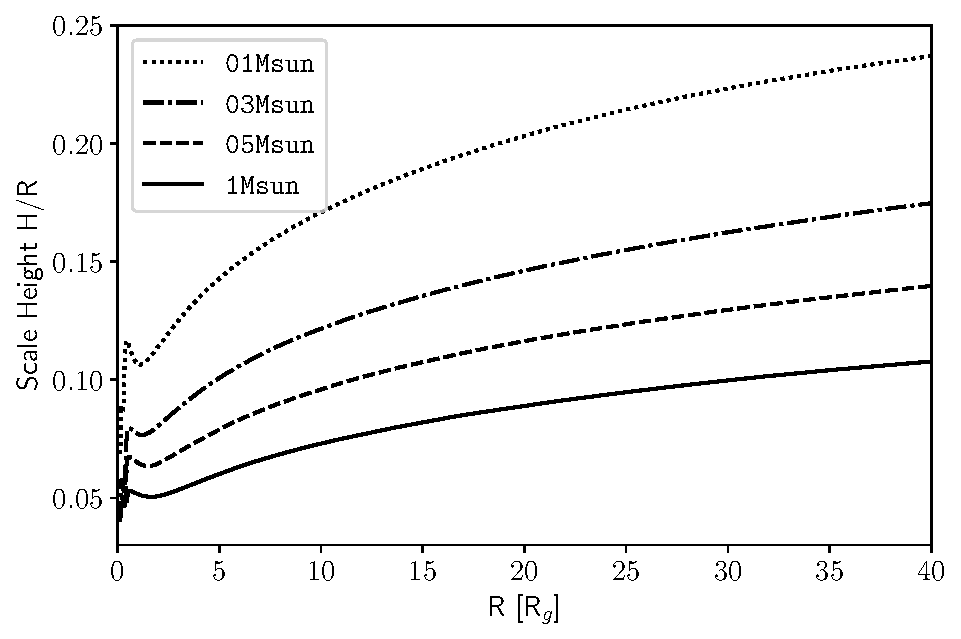
\includegraphics[width=\columnwidth]{Figure5}
    \caption{Initial disc aspect ratio for the runs reported in Tab.~\ref{tab:stars}. \label{fig:aspectratio}}
\end{figure}
Two main aspects can be seen in the observed profiles. 
(i) The disc aspect ratio is strongly dependant on the stellar mass, and it is not affected by the X-ray photoevaporation (comparing the bottom panels of Figures \ref{fig:discs} and \ref{fig:initdiscs}), which cannot reach the deeper dense regions of the disc until the mass accretion rate becomes comparable to the photoevaporative rate. We show this in a more quantitative way in Figure~\ref{fig:aspectratio}, where we plot the disc aspect ratio as a function of radius for the different stellar masses. Within \SI{40}{R_g} the disc flaring changes from \SI{0.1}{\solarmass} with a disc aspect ratio of $h/r = 0.096 \cdot r^{0.25}$ to \SI{1}{\solarmass} with $h/r = 0.036 \cdot r^{0.3}$. The larger disc flaring for low stellar masses affects the vertical location of the maximum penetration depth of X-rays (shown in Figure~\ref{fig:discs} as a red dashed line) which shifts further away from the disc mid-plane.
(ii) The temperature structure in the wind region, even when rescaled by the gravitational radius, varies considerably for the different stellar masses, in contrast to what predicted analytically in \citetads{2012MNRAS.422.1880O}, showing warmer winds for larger stellar masses and X-ray luminosities.

\subsection{Mass-loss rates}\label{sec:mdot}
We integrated the gas flow along the streamlines in the wind during the last \SI{50}{orbits} of each simulation and plotted the resulting cumulative mass-loss rates as a function of stellar masses in a square-box plot in Figure~\ref{fig:Mdot}, where we included also the run with a \SI{0.7}{\solarmass} star from \citetalias{2019MNRAS.487..691P}, which has been rescaled in order to have the same stellar mass--X-ray luminosity adopted in these runs following eq.~\ref{eq:Lx}.
\begin{figure}
  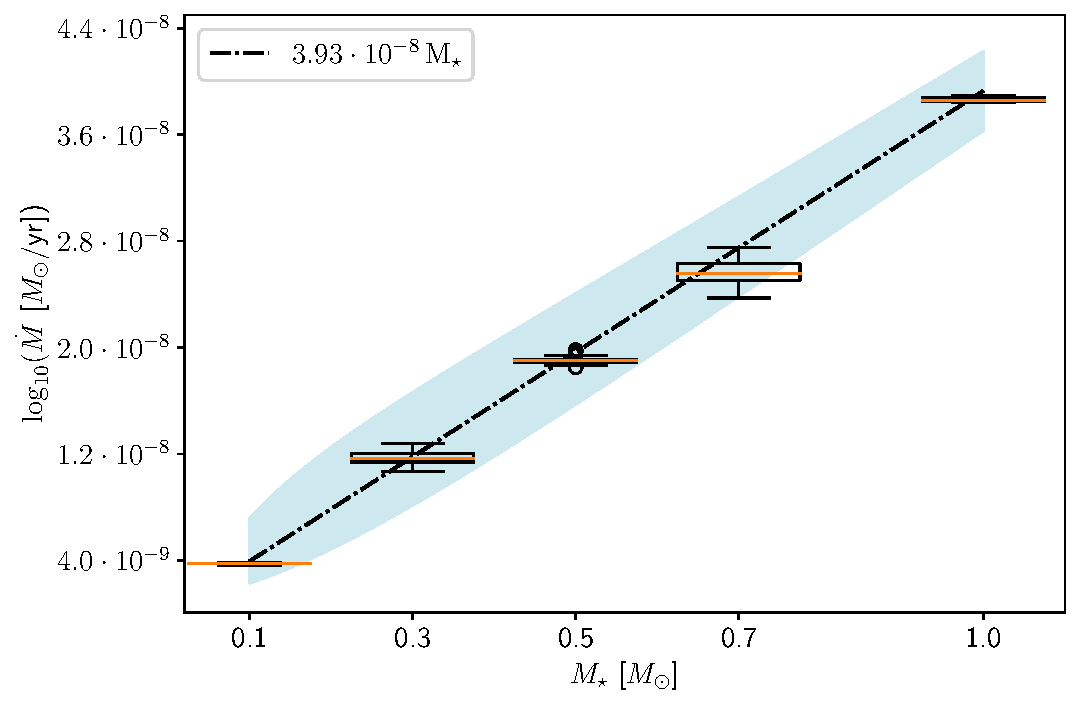
\includegraphics[width=\columnwidth]{Figure6}
  \caption{Box plot of the cumulative mass-loss rate as a function of stellar mass over the last $50$ orbital timescales at \SI{10}{\astronomicalunit}. The derived linear fit is overplotted with a black dashed line, and a blue shaded region shows the variation in the mass-loss rate due to the uncertainty in the X-ray luminosity as a function of stellar mass in equation~\ref{eq:Lx}. \label{fig:Mdot}}
\end{figure}
A fitting function has been overplotted with a dashed line, which shows the linear dependence of the mass-loss rate as a function of stellar mass. This linear trend is in contrast with the flat distribution as a function of stellar mass ($\propto \mathrm{M}_\star^{-0.068}$) obtained by \citetads{2012MNRAS.422.1880O}, but there the X-ray luminosity was kept constant while changing the stellar mass (see Section~\ref{sec:mass-dependance} for a proper comparison). Furthermore, the linear trend doesn't show the flattening of the mass-loss rates observed for large X-ray luminosity in \citetalias{2019MNRAS.487..691P} because even the \SI{1}{\solarmass} star has an X-ray luminosity of $\log(L_X) = 30.3$, which is smaller than the saturation value observed in the previous study.
The best fitting function obtained from the current study is
\begin{equation}\label{eq:MdotLxMass}
  \dot{\mathrm{M}}_w = 3.93\times10^{-8} \left(\frac{\mathrm{M}_\star}{\si{\solarmass}}\right) [\si{\solarmass.yr^{-1}}]\,.
\end{equation}
%We show in Figure~\ref{fig:Mdot} with a shaded light blue region the influence of the $1 \sigma$ error reported in eq.~\ref{eq:Lx} on the cumulative mass-loss rate following the relation derived in \citetads{2019MNRAS.487..691P}
%\begin{equation}\label{eq:MdotLx}
%  \log_{10}(\dot{\mathrm{M}}(L_X)) = A_\textrm{L} \exp{\left[\frac{(\ln{(\log_{10}(L_X))}-B_\textrm{L})^2}{C_\textrm{L}}\right]} + D_\textrm{L} [M_\odot\, \mathrm{yr}^{-1}]\,,
%\end{equation}
%with $A_\textrm{L} = -2.7326$, $B_\textrm{L} = 3.3307$, $C_\textrm{L} = -2.9868\cdot10^{-3}$, $D_\textrm{L} = -7.2580$.

\subsection{Wind profiles}\label{sec:wind-prof}
From the derivative of the integrated mass-loss profile along the cylindrical radius we obtain the radial distribution of the mass-loss rate shown in Figure~\ref{fig:Sigmadot}. Looking at the top panel, two trends are visible. There is an increase of the peak location as a function of stellar mass, with the only exception for the \SI{0.3}{\solarmass} star. A similar increase is seen in the maximum reach of the wind in the outer regions of the protoplanetary disc, which is able to remove material up to \SI{\sim 35}{\astronomicalunit} for a \SI{0.1}{\solarmass} star, while it reaches \SI{\sim 270}{\astronomicalunit} for a \SI{1}{\solarmass} star. This is a direct result of the lower flaring for disc orbiting larger mass stars, which allows the wind to have a further reach in the outer disc regions and generate a more massive wind.

To understand the anomaly observed for the \SI{0.3}{\solarmass} star we rescaled the cylindrical radius by the gravitational radius in the bottom panel of Figure~\ref{fig:Sigmadot}.
We can see that, when rescaled, we obtain 2 similar profiles for the low X-ray luminosities (and spectra hardness) and two for the high luminosities. This can be explained with the harder spectra in the 'soft' X-ray band (0.1–1 keV) for lower X-ray luminosities which drives the peak at larger radii, as studied in \citetalias{Ercolano2021}. The relative difference amongst the profiles, once rescaled, is given by a combined effect of the change in the stellar mass and absolute value of the X-ray luminosity.
\begin{figure}
  \centering
  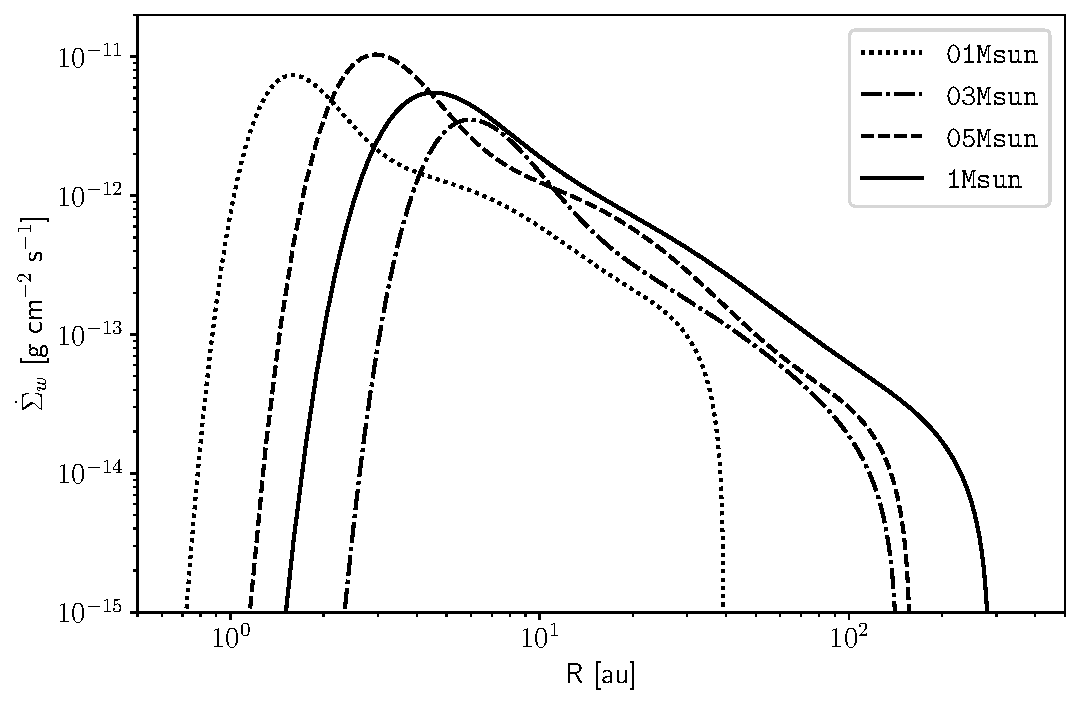
\includegraphics[width=\columnwidth]{Figure7a}
  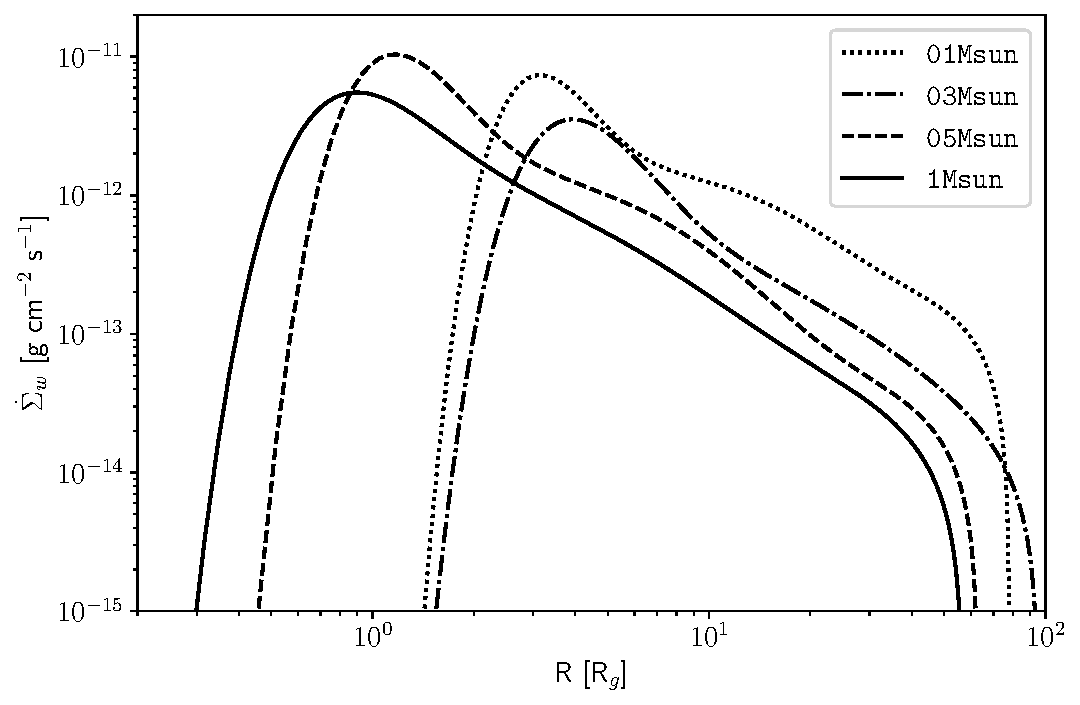
\includegraphics[width=\columnwidth]{Figure7b}
  \caption{Surface density mass-loss rate profile for the different simulations. In the top panel the mass-loss rate is plotted as a function of the cylindrical radius in au, while in the bottom panel the dependence is a function of the gravitational radius (see section~\ref{sec:wind-prof}). \label{fig:Sigmadot}}
\end{figure}

The best fit for the surface mass-loss rate is given by the following function, as in \citetalias{2019MNRAS.487..691P}
\begin{eqnarray}
  \dot{\Sigma}_w(R) &= \ln{(10)} \bigg(\frac{6\, a\, \ln{(R)}^5}{R\, \ln{(10)}^6} +
  \frac{5\, b\, \ln{(R)}^4}{R\, \ln{(10)}^5} +
  \frac{4\, c\, \ln{(R)}^3}{R\, \ln{(10)}^4} + \\ \nonumber
  &\frac{3\, d\, \ln{(R)}^2}{R\, \ln{(10)}^3} +
  \frac{2\, e\, \ln{(R)}}{R\, \ln{(10)}^2} + \\ \nonumber
  &\frac{f}{R\, \ln{(10)}}\bigg)
  \frac{\dot{\mathrm{M}}_w(R)}{2\pi\, R} \ [\SI{}{\solarmass.\astronomicalunit^{-2}.yr^{-1}}]\,
\end{eqnarray}
where
\begin{equation}
  \frac{\dot{\mathrm{M}}_w(R)}{\dot{\mathrm{M}}_w(\mathrm{L}_X)} = 10^{a\log{R}^6 + b\log{R}^5 + c\log{R}^4 + d\log{R}^3 + e\log{R}^2 + f\log{R} + g}
\end{equation}
where the parameters for the different stellar masses are given in Table~\ref{tab:fit}.
\begin{table*}
\caption{Parameters for the Surface density profiles}
\label{tab:fit}
\centering
\begin{tabular}{c c c c c c c c c}
\hline
$\mathrm{M}_\star$ [\si{\solarmass}] & a & b & c & d & e & f & g & $\dot{\mathrm{M}}_w$ [\SI{e-8}{\solarmass.\year^{-1}}]\\
\hline
\hline
   $1.0$ & $-0.6344$ & $6.3587$ & $-26.1445$ & $56.4477$ & $-67.7403$ & $43.9212$ & $-13.2316$ & $3.86446$\\
   $0.5$ & $-1.2320$ & $10.8505$ & $-38.6939$ & $71.2489$ & $-71.4279$ & $37.8707$ & $-9.3508$ & $1.9046$\\
   $0.3$ & $-1.3206$ & $13.0475$ & $-53.6990$ & $117.6027$ & $-144.3769$ & $94.7854$ & $-26.7363$ & $1.17156$\\
   $0.1$ & $-3.8337$ & $22.9100$ & $-55.1282$ & $67.8919$ & $-45.0138$ & $16.2977$ & $-3.5426$ & $0.37588$\\
\hline
\end{tabular}
\end{table*}

\subsection{Stellar mass dependence}\label{sec:mass-dependance}
In order to isolate the effect of stellar mass on the photoevaporative mass-loss rates we performed a new set of simulations where we kept constant the X-ray luminosity to the value of \SI{7e29}{erg.s^{-1}} (that of the \SI{0.5}{\solarmass} star) while changing only the stellar mass.
%The resulting surface mass-loss rate is reported in Figure~\ref{fig:SigmadotMtest} where we can isolate the effect of the stellar mass on the shift of the peak, due to the increasing gravitational pull which prevents the thermal wind to leave the disc. Furthermore, the different disc flaring as a function of stellar mass is responsible of the increased reach of the stellar wind, that can remove material up to 300 au for 1 Solar mass star.
%\begin{figure}
%  \centering
%  \includegraphics[width=0.5\textwidth]{Sigmadot_Mtest}
%  \caption{Surface density mass-loss rate profile as a function of cylindrical radius for 3 different stellar masses but with the same X-ray luminosity \label{fig:SigmadotMtest}.}
%\end{figure}
We show in Figure~\ref{fig:cumdotMtest} the cumulative mass-loss rate for the different stellar masses and we compare it with the prescription from \citetads{2012MNRAS.422.1880O}.
\begin{figure}
  \centering
  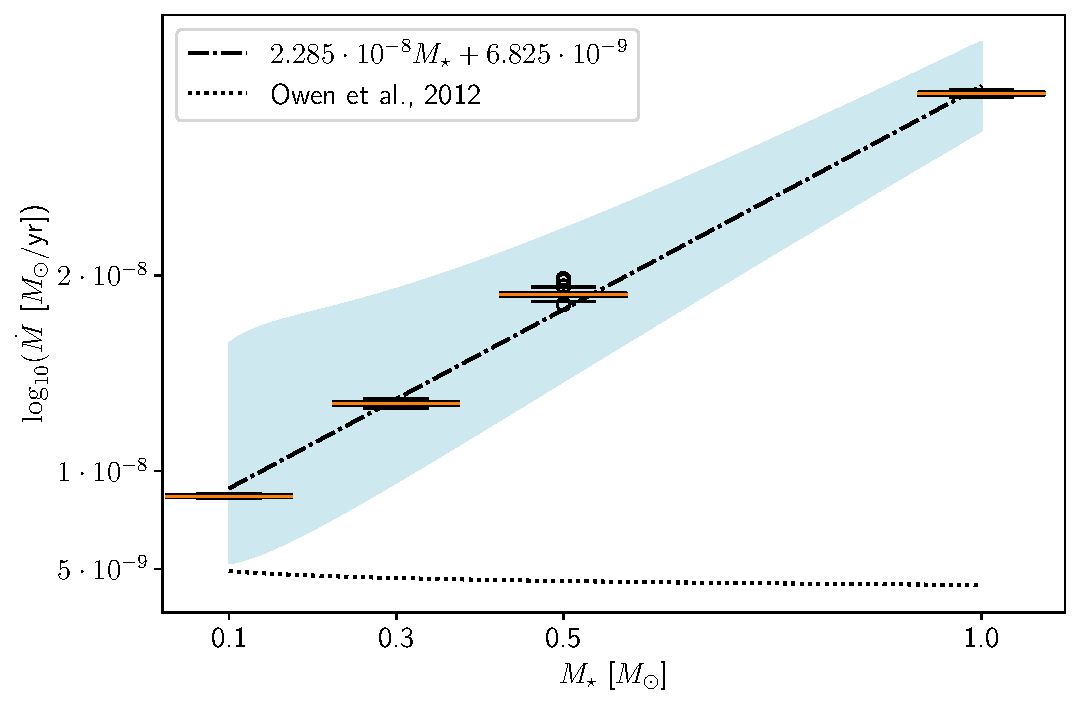
\includegraphics[width=\columnwidth]{Figure8}
  \caption{Box plot of the cumulative mass-loss rate as a function of stellar mass over the last 50 orbital timescales at \SI{10}{\astronomicalunit}, keeping the X-ray luminosity fixed. A linear fit has been overplotted with a dot-dashed line, as well as the prediction from \citepads{2012MNRAS.422.1880O} in a dotted line. \label{fig:cumdotMtest}}
\end{figure}
We see that also in this case the mass-loss rate is not flat, in contrast to what was observed in \citetads{2012MNRAS.422.1880O}. The reason is again the difference in the disc flaring which allows larger mass stars to reach further regions in the disc, generating a large mass flux. However, the dependence of the mass-loss rate as a function of the pure stellar mass becomes much more shallow, increasing only by a factor $3$ from \SI{0.1}{\solarmass} to \SI{1}{\solarmass} instead of an order of magnitude as shown in Figure~\ref{fig:Mdot}.
The linear fit that matches the data shown in Figure~\ref{fig:cumdotMtest} is
\begin{equation}
    \dot{\mathrm{M}}_w = 2.34 \times 10^{-8} \left(\frac{\mathrm{M}_\star}{\si{\solarmass}}\right) + 6.23 \times 10^{-9}\,.
\end{equation}

%\subsection{Disc structure and gas streamlines}\label{sec:streamlines}
%The topology of the gas streamlines is strongly dependent on the underlying disc structure. This behaviour has already been studied in the context of transitional discs \citepalias[see e.g.][]{2019MNRAS.487..691P}, where at the inner edge of the disc the gas streamlines are moving inwards before curving and leave the disc radially.
%In Figure~\ref{fig:streamlines} we show the gas streamlines for the $0.1 \mathrm{M}_\star$ for which this effect is stronger. There is a change in the direction of the streamline curvature at the base of the flow corresponding to a change in the sign of the disc aspect ratio gradient, as shown in Figure~\ref{fig:hr}.
%While for $r<r_g\sim 0.3$ au the gas is still gravitationally bound, the stellar irradiation can move it to larger radii where it can leave the system. As a result, inside $0.3$ au the gas is moving outwards, while outside it is accelerating moving inwards before leaving radially the disc, creating around $0.3$ au a maximum in the profile for the surface mass-loss rate.
%\begin{figure}
%    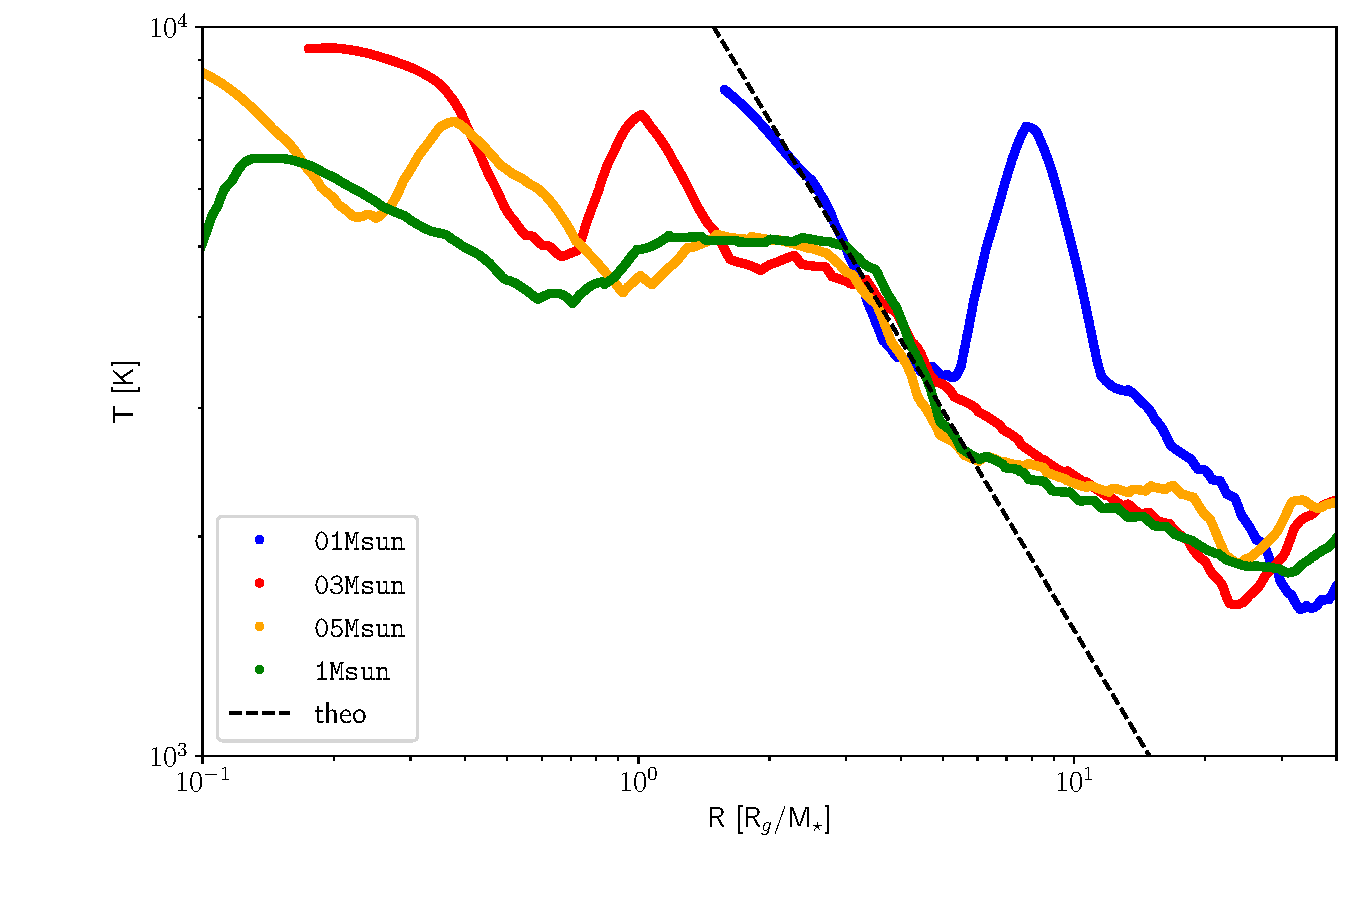
\includegraphics[width=0.45\textwidth]{Tss}
%    \caption{Temperature at the disc launching region. \label{fig:Twind}}
%\end{figure}
%This effect is much stronger for low stellar luminosities, as highlighted in the inset of Figure~\ref{fig:hr}.
%\begin{figure}
%    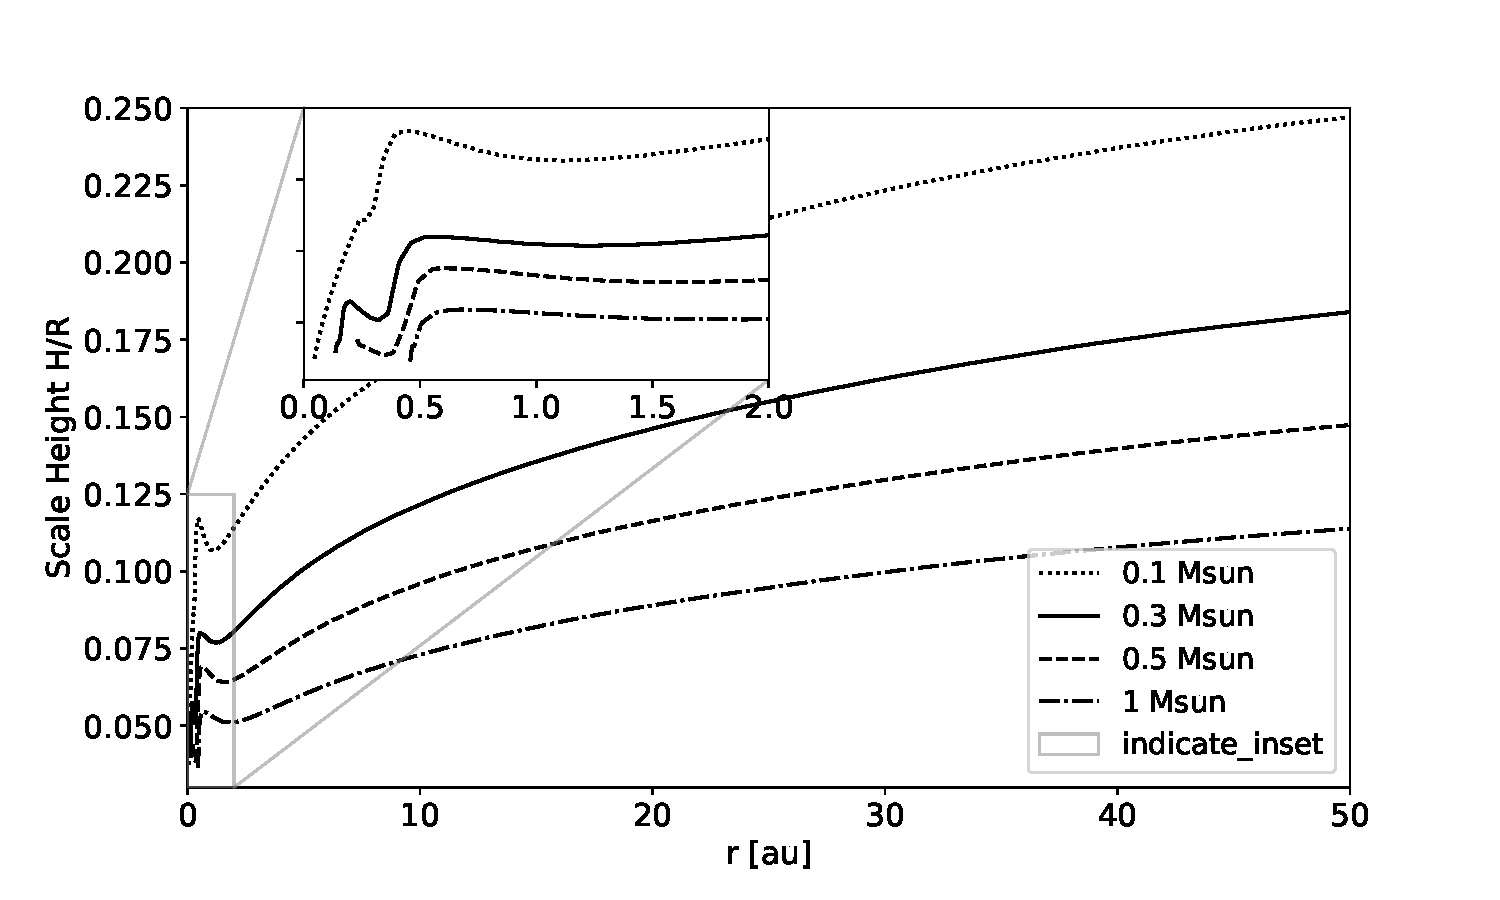
\includegraphics[width=0.5\textwidth]{HR_comp}
%    \caption{Disc aspect ratio in the inner 50 au of the different runs performed. In the inset a zoom in on the inner 2 au is shown to highlight the change in the sign of the aspect ratio gradient which is related to a change in the topology of the streamlines at the base of the flow. \label{fig:hr}}
%\end{figure}
%The final disc density distribution for the different stellar masses (and luminosities) is shown in Figure~\ref{fig:discs} where the strong increase in the disc aspect ratio as a function of stellar mass is highlighted.

%The larger flare in the disc structure for low stellar masses compensates the lower penetration depth of the high energetic X-ray irradiation, producing only a modest difference in the final cumulative mass-loss rate.

%The self-similarity of gas streamlines across different stellar masses proposed by
%\citetads{2012MNRAS.422.1880O} is then lost both close to the disc surface because of the different curvature of the streamlines, and also at larger radii due to the increase of the disc aspect ratio as a function of stellar mass and luminosity.


%\subsection{Inner boundary}\label{sec:inner-boundary}

%The inner boundary of the simulation domain plays a crucial role as the outer one, explored in depth in \citep{2019MNRAS.487..691P}. We study in detail the variation of the photoevaporation profile changing the

%\subsection{Sonic surface}\label{sec:sonic-surface}
%The analysis of \citetads{2012MNRAS.422.1880O} is based on the assumption that the properties of the mass-flux can be determined at the sonic surface, and that the sound speed is roughly given by the Parker value
%\begin{equation}
%  c_s^2 = \frac{G\mathrm{M}_\star}{2R}
%\end{equation}
%An important assumption is that the height of the sonic surface is not much larger than its cylindrical radius ($z_s \ngg R$), which can brake down for lower stellar masses, since the disc flaring is proportional to the central mass.

%-------------------------------------------------------------------
\section{Discussion}\label{sec:discussion}
%-------------------------------------------------------------------

In this section we discuss the differences between the properties at the sonic surface in our model in comparison with the theoretical prediction for a Parker wind and previous numerical results. We then compare the disc life-time obtained from our model with observationally derived inner disc lifetimes.

\subsection{Sonic surface}
The local gas properties at the sonic surface are fundamental to understand the overall wind properties.
For a disc wind, the sound speed at the sonic surface should be on the same order of magnitude of the Parker value which, from equation~\ref{eq:rcrit}, is
\begin{equation}
    {c_s}^2 \approx \frac{G \mathrm{M}_\star}{2R}\,.
\end{equation}
In Figure~\ref{fig:sonicsurf} we plot the density (upper plot) and temperature (bottom plot) at the sonic surface for the different runs, and we compare the temperature with the theoretical prediction for a Parker wind.
We see that in our case the steepness of the temperature profile is much shallower, and only the \SI{1}{\solarmass} star (green line) matches the expected profile between $3$ and $6$ gravitational radii before flattening again.
\begin{figure}
    \centering
    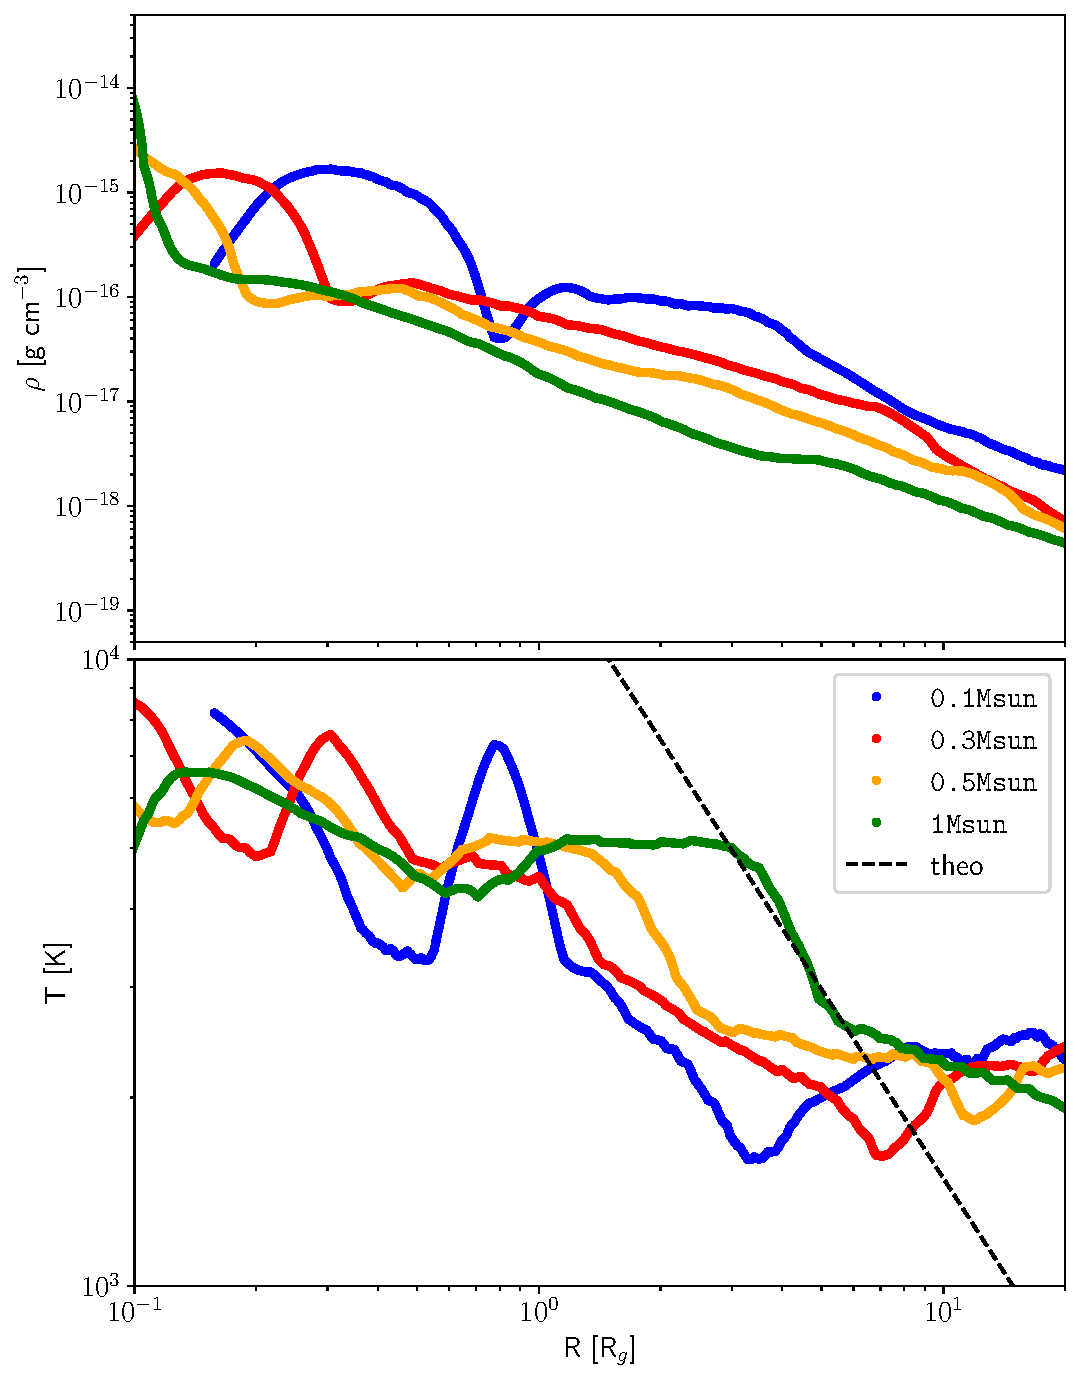
\includegraphics[width=\columnwidth]{Figure9}
    \caption{Temperature at sonic surface as a function of the gravitational radius for the different stellar masses modelled. \label{fig:sonicsurf}}
\end{figure}
This behaviour has been observed also by \citeads{2012MNRAS.422.1880O} (see their Figure 6), where the Parker wind value was recovered only around the gravitational radius, flattening close to the star and far away from it, following the sigmoidal temperature prescription coming from Figure~\ref{fig:tempxi}.
Two trends can be identified in Figure~\ref{fig:sonicsurf}.
(i) The density at the sonic surface is almost linearly increasing with stellar mass, being \SI{9.2e-17}{g.cm^{-3}} for the \SI{0.1}{\solarmass} star and \SI{6.5e-18}{g.cm^{-3}} for \SI{1}{\solarmass}. The bump observed inside $\mathrm{R}_g$ is caused by the bump in the disc scale height from Figure~\ref{fig:aspectratio}, which comes directly from the \textsc{diad} models and is caused by an increase of the dust temperatures close to the star.
(ii) The temperature passes through a transition regime with a similar slope which is shifted towards the central star going from the higher to the lower mass star. This shift is also linearly increasing with the stellar mass, and to show it, we replot the bottom panel of Figure~\ref{fig:sonicsurf} dividing the gravitational radius again by the stellar mass in Figure~\ref{fig:sonicsurfrescaled}, where the theoretical temperature for the \SI{1}{\solarmass} star is reported to guide the eye.
\begin{figure}
    \centering
    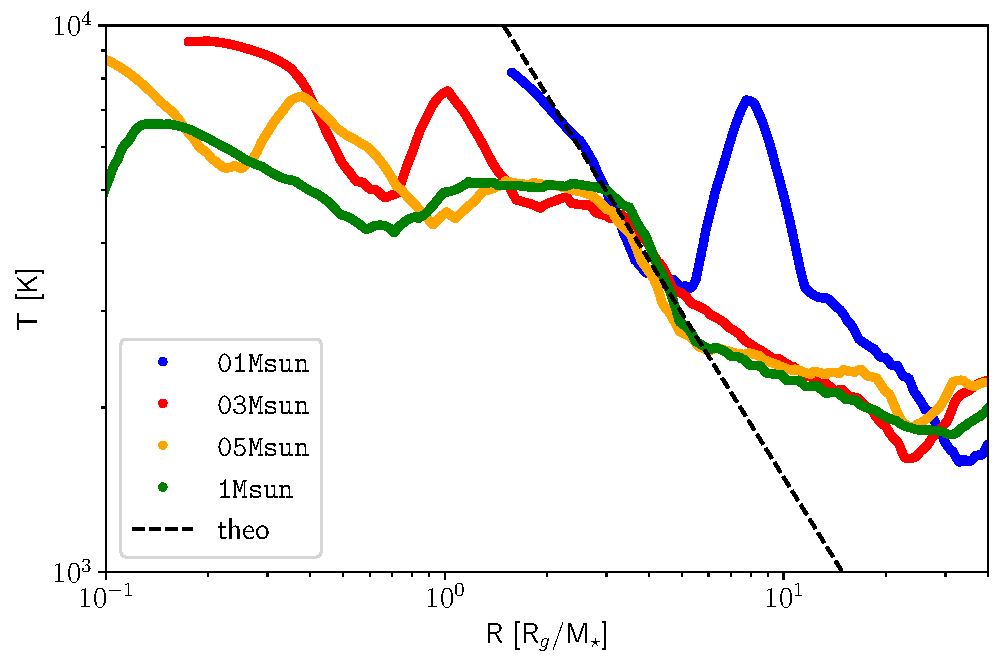
\includegraphics[width=\columnwidth]{Figure10}
    \caption{Temperature at sonic surface as a function of the gravitational radius divided by the stellar mass for the different models. \label{fig:sonicsurfrescaled}}
\end{figure}
The linear radial shift in the temperature at the sonic surface may be due to the difference in the disc scale height, which affects the density at the sonic surface, and thus the ionization parameter which is responsible for the change in the temperature. 

\subsection{Observational constraints}
The observed lifetimes of disks around stars of different masses presents a fundamental constraint for disk dispersal models. Our new models which span the observational range of observed stellar masses in disc surveys allow us to make the first such comparison for a disc-dispersal model.

We can define the inner disc life-time $t_\mathrm{life}$ as the time at which accretion rates $\dot{\mathrm{M}}_\mathrm{acc}$ decrease to photoevaporative rates $\dot{\mathrm{M}}_w$.
This happens because, at this time, a gap opens in the inner disc (around the gravitational radius) disconnecting the inner and outer disc evolution. 
The inner disc disperses on a short timescale (viscous timescale at few \si{\astronomicalunit}), not being replenished anymore by the outer disc.
The lifetime of the inner disc $t_\mathrm{life}$ can be approximated then by
\begin{equation}\label{eq:tlifedef}
    \dot{\mathrm{M}}_w = \dot{\mathrm{M}}_\mathrm{acc,0}\left(\frac{t_\mathrm{life}}{t_\nu}\right)^{-3/2}\, ,
\end{equation}
where $t_\nu$ is the viscous timescale
\begin{equation}
    t_\nu = \frac{M_\mathrm{disc,0}}{2 \dot{\mathrm{M}}_\mathrm{acc,0}}\, .
\end{equation}
Combining the previous equations we obtain
\begin{eqnarray}\label{eq:tlife}
    t_\mathrm{life} &=& t_\nu \left(\frac{\dot{\mathrm{M}}_\mathrm{acc,0}}{\dot{\mathrm{M}}_w}\right)^{2/3} = \frac{M_\mathrm{disc,0}}{2 \dot{\mathrm{M}}_\mathrm{acc}}\left(\frac{\dot{\mathrm{M}}_\mathrm{acc}}{\dot{\mathrm{M}}_w}\right)^{2/3} \nonumber \\
    &=& \frac{1}{2}\left(\frac{M_\mathrm{disc,0}}{\dot{\mathrm{M}}_\mathrm{acc,0}^{1/3}\,\dot{\mathrm{M}}_w^{2/3}}\right)\, ,
\end{eqnarray}
where the free parameters are given by the initial disc mass and accretion rates.
For several star forming regions an observational $\dot{\mathrm{M}}_\mathrm{acc}-\mathrm{M}_\star$ relation has been determined (\citeads{2017A&A...600A..20A}, \citeads{2017A&A...604A.127M}, \citeads{2021A&A...648A.121F}, \citeads{2021A&A...652A..72A}), where, like in the $1$ to \SI{3}{\mega\year} old Lupus, a sharp increase of the accretion rate is observed for low-mass stars ($<$\SI{0.2}{\solarmass}, \citeads{2017A&A...600A..20A})
\begin{equation}\label{eq:mdotAlcala}
    \log(\dot{\mathrm{M}}_\mathrm{acc}) = 
    \begin{cases}
      4.58 (\pm 0.68) \, \log(\mathrm{M}_\star) - 6.11(\mp 0.61), & \leq \SI{0.2}{\solarmass} \\
      1.37 (\pm 0.24) \, \log(\mathrm{M}_\star) - 8.46 (\mp 0.11), & \text{otherwise.}
    \end{cases}
\end{equation}
We can then use the current accretion rates to determine the initial accretion rate, assuming a constant disc viscous evolution
\begin{equation}\label{eq:mdot0}
    \dot{\mathrm{M}}_\mathrm{acc} = \dot{\mathrm{M}}_\mathrm{acc,0} \left(\frac{t}{t_\nu}\right)^{-3/2}\,,
\end{equation}
which leaves us only with the free parameter of the initial disc mass $M_\mathrm{disc,0}$.

%\citetads{2016ApJ...831..125P} and \citetads{2021arXiv210605247R} found also a steeper than linear relation between the dust disc mass and the stellar mass.
%\begin{equation}
%    M_\mathrm{disc}= M_\mathrm{disc,0} \left(\frac{\mathrm{M}_\star}{\si{\solarmass}}\right)^{\alpha}\,,
%\end{equation}
%with $\alpha = [1.31 \pm 0.24, 1.10 \pm 0.30, 1.73 \pm 0.39]$ for the Taurus, Lupus, and Upper Sco star forming regions respectively.
An interesting star forming region to test the validity of our observational predictions is $\lambda$-Orionis (also known as Collinder~$69$), since it has been extensively studied in X-ray emission \citepads{2011A&A...526A..21B}, and it seems to be at a critical age for disc dissipation (\SI{\sim 5}{\mega\year}).
\citeads{2012A&A...547A..80B} obtained the cumulative disc fraction as a function of stellar mass from infrared excess observations of this open cluster, and we can convert this into an approximate disc lifetime, following the approach of \citeads{2021ApJ...910...51K} as
\begin{equation}
    t_\mathrm{life} \simeq -\frac{t_\mathrm{age}}{\ln{f_\mathrm{disc}}}\, ,
\end{equation}
where $t_\mathrm{age} = 5\, \mathrm{Myr}$ \citepads{2011A&A...536A..63B}.

In Fig.~\ref{fig:obs} we directly compared the observational data points derived from \citetads{2012A&A...547A..80B} in grey, with the disc lifetime obtained from eqs.~\ref{eq:MdotLxMass}, \ref{eq:tlife} in sea-green and, for comparison, in light-green the result using the photoeavaporative mass-loss rate from eq.~B1 of \citetads{2012MNRAS.422.1880O}. The shaded region represents the uncertainty in the observational relation between the accretion rates and stellar masses.

In order to get the best fit to the observation we used a linear relation between the initial disc mass and stellar mass and a initial value of \SI{0.14}{\mathrm{M}_\star} for the current models and \SI{0.06}{\mathrm{M}_\star} for \citetads{2012MNRAS.422.1880O}.
\citetads{2013ApJ...771..129A} found a roughly linear relationship between the disc mass and stellar mass, studying a large sample of Class~II discs. More recently \citetads{2016ApJ...831..125P}, studying a few young star forming regions, found a slightly steeper than linear dust disc mass - stellar mass relationship, though including in the sample also the brown dwarfs linearizes it again \citepads{2021arXiv210605247R}.
\begin{figure}
    \centering
    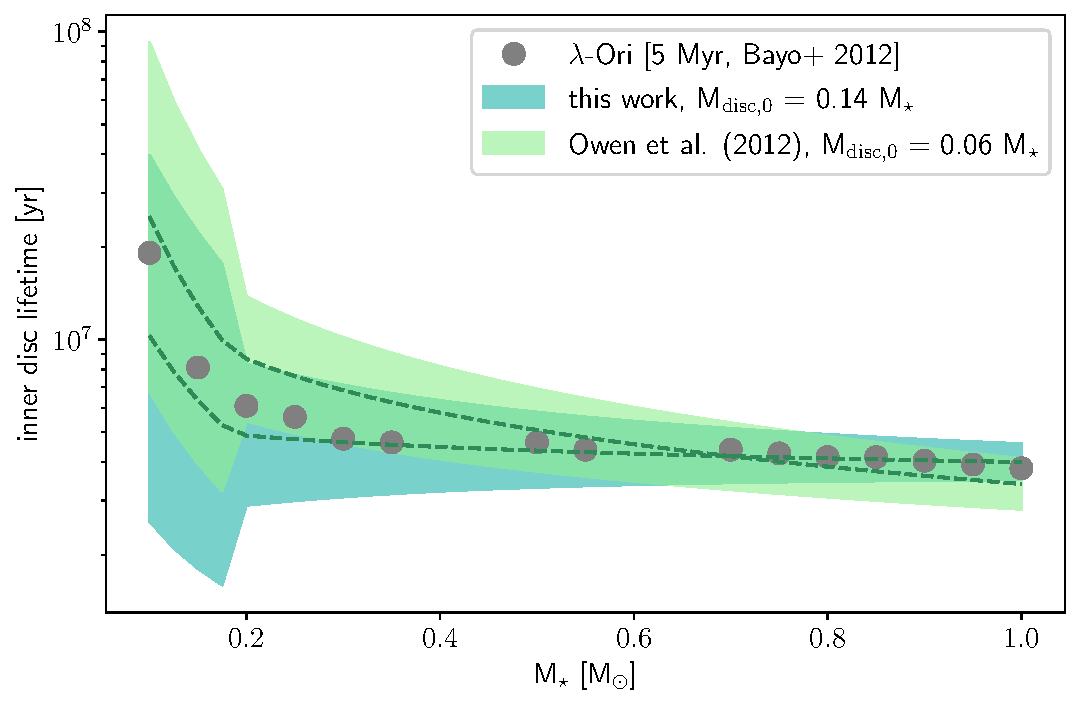
\includegraphics[width=\columnwidth]{Figure11}
    \caption{Inner disc lifetime calculated from our models using eq.~\ref{eq:tlife} compared with the disc fraction as a function of the mass for the members of $\lambda$-Ori. The shaded regions show the uncertainty in equations~\ref{eq:mdotAlcala},\ref{eq:Lx}. \label{fig:obs}}
\end{figure}
The results match very well the observations for the whole range of explored masses, and in particular the change in the slope for masses below \SI{0.3}{\solarmass}, which gives us confidence on the ability of the photoevaporative models to predict the observed disc lifetimes. Furthermore, our new prescription, with a linear scaling of disc masses as a function of stellar mass, captures better the disc lifetime distribution with respect to the previous state of the art model.

%-------------------------------------------------------------------
\section{Conclusions}\label{sec:conclusions}
%-------------------------------------------------------------------

  We have computed for the first time comprehensive photo-evaporation models spanning the whole observed range of low mass stars ($\leq$ \SI{1}{\solarmass}) using observationally derived X-ray stellar spectra. 
  We found that

   \begin{enumerate}
      \item stellar mass and irradiation have a strong impact on the underlying disc structure, changing the disc aspect ratio and causing a large flaring for low X-ray luminosities/small masses, which affects the density and temperature in the wind region (see Figure~\ref{fig:discs});
      \item we provide fitting functions in Table~\ref{tab:fit} for the surface mass-loss rate profiles for different stellar masses whose luminosity is scaled based on equation~\ref{eq:Lx} that can be readily applied to disc and planet population synthesis codes;
      \item the resulting cumulative mass loss rate scales linearly with the stellar mass (see equation~\ref{eq:MdotLxMass});
      \item the temperature as a function of the gravitational radius at the sonic surface scales linearly with the stellar mass (see Figure~\ref{fig:sonicsurfrescaled});
      \item the observed disc lifetimes as a function of stellar mass can be very well reproduced by our new models, indicating that X-ray photo-evaporation dominates the final phases of protoplanetary disk evolution (see Figure~\ref{fig:obs}).
   \end{enumerate}

\section{Data availability}
   The data underlying this article and the scripts used to create the Figures are available at \href{https://cutt.ly/lElY9JI}{https://cutt.ly/lElY9JI}.

\section*{Acknowledgements}

    GP acknowledges support from the DFG Research Unit ‘Transition Disks’ (FOR 2634/1, ER 685/8-1).
    This work was performed on the computing facilities of the Computational Center for Particle and Astrophysics (C2PAP).
    This research was supported by the Excellence Cluster ORIGINS which is funded by the Deutsche Forschungsgemeinschaft (DFG, German Research Foundation) under Germany's Excellence Strategy - EXC-2094 - 390783311.
    This paper utilizes the D’Alessio Irradiated Accretion Disk (DIAD) code. We wish to recognize the work of Paola D’Alessio, who passed away in 2013. Her legacy and pioneering work live on through her substantial contributions to the field.

\bibliographystyle{mnras}
\bibliography{biblio}

% Don't change these lines
\bsp	% typesetting comment
\label{lastpage}
\end{document}
